\section{译者补充:微面模型相关推导}\label{sec:译者补充:微面模型相关推导}
\begin{remark}
    本节内容不是原书内容,而是译者根据\citet{heitz:hal-01024289}、
    \citet{1138991}、\citet{1142437}和\citet{10.5555/2383847.2383874}整理
    并推导后补充的,请酌情参考和斧正。
\end{remark}
\subsection{微面分布函数的定义与性质}\label{sub:微面分布函数的定义与性质}
如\reffig{08ex01-macrosurfaceMicrosurface},我们考虑一个足够小的宏曲面$\mathcal{G}$,设它是个绝对光滑的平面,具有法线$\bm n$.
微面模型中,真正粗糙起伏的曲面,即微曲面$\mathcal{M}$,是由许多偏离宏曲面的微面构成的。
或者说,微曲面$\mathcal{M}$上所有的点在方向$\bm n$上投影即得$\mathcal{G}$.
将宏曲面上的点记为${\bm p}_{\mathrm{g}}$,其周围的微分面元为$\mathrm{d}{\bm p}_{\mathrm{g}}$,
则宏曲面的面积为
\begin{align}
    S=\int\limits_{\mathcal{G}}\mathrm{d}{\bm p}_{\mathrm{g}}\, .
\end{align}

将$\mathcal{M}$上的点记作${\bm p}_{\mathrm{h}}$,该点处的法线记作${\bm\omega}_{\mathrm{h}}({\bm p}_{\mathrm{h}})$.
引入三维意义下的狄拉克$\delta$分布,
它满足$\displaystyle\int\limits_{\varOmega}\delta({\bm\omega})\mathrm{d}{\bm\omega}=1$.
并记$\delta_{\bm\omega}({\bm\omega}')=\delta({\bm\omega}'-{\bm\omega})$.
由此定义\keyindex{微面分布函数}{microfacet distribution function}{distribution分布}为
\sidenote{原论文全文假定$S=1$来讨论,不用除以面积,这里笔者的处理有所不同。}
\begin{align}\label{eq:08ex01-MicrosurfaceDistribution}
    D({\bm\omega})=\displaystyle\frac{1}{S}\int\limits_{\mathcal{M}}
    \delta_{\bm\omega}({\bm\omega}_{\mathrm{h}}({\bm p}_{\mathrm{h}}))
    \mathrm{d}{\bm p}_{\mathrm{h}}\, ,
\end{align}
其中狄拉克$\delta$分布和$D({\bm\omega}_{\mathrm{h}})$的量纲均为
球面度的倒数即$\displaystyle\frac{1}{\text{sr}}$,也相当于无量纲。

\begin{figure}[htbp]
    \centering
    \includegraphics[width=0.6\linewidth]{Pictures/chap08/macrosurfaceMicrosurface.eps}
    \caption{宏曲面(黑色)与微曲面(红色)。}
    \label{fig:08ex01-macrosurfaceMicrosurface}
\end{figure}

我们可以把${\bm\omega}_{\mathrm{h}}$视作从$\mathcal{M}$到整个方向空间$\varOmega$的映射。
注意$\varOmega$包含了球心到完整球面上任意一点的所有可能方向(总立体角为$4\pi$,尽管该映射不一定能覆盖全)。
现在考虑$\mathcal{M}$和$\varOmega$各自的子集$\mathcal{M'}$和$\varOmega'$,
并设它们满足以下条件:点${\bm p}_{\mathrm{h}}$属于$\mathcal{M'}$当且仅当
该点处的微面法线${\bm\omega}_{\mathrm{h}}({\bm p}_{\mathrm{h}})$属于$\varOmega'$,即
\begin{align}
    {\bm p}_{\mathrm{h}}\in\mathcal{M'}\Leftrightarrow
    {\bm\omega}_{\mathrm{h}}({\bm p}_{\mathrm{h}})\in\varOmega'\, .
\end{align}
由此利用积分换元可得微面分布函数具有计算指定微曲面面积的能力:
\begin{align}
    \label{eq:08ex01-microsurfaceArea}
    \int\limits_{\mathcal{M}'}\mathrm{d}{\bm p}_{\mathrm{h}}
    =S\int\limits_{\varOmega'}D({\bm\omega}_{\mathrm{h}})\mathrm{d}{\bm\omega}_{\mathrm{h}}\, .
\end{align}
而整个微曲面面积就是
\begin{align}
    \int\limits_{\mathcal{M}}\mathrm{d}{\bm p}_{\mathrm{h}}
    =S\int\limits_{\varOmega}D({\bm\omega}_{\mathrm{h}})\mathrm{d}{\bm\omega}_{\mathrm{h}}\, .
\end{align}

进一步地,对于任意关于微面法线的函数$f({\bm\omega}_{\mathrm{h}})$,
利用$D({\bm\omega}_{\mathrm{h}})$可将空间积分与统计积分相互转化:
\begin{align}
    \int\limits_{\mathcal{M}}f({\bm\omega}_{\mathrm{h}}({\bm p}_{\mathrm{h}}))\mathrm{d}{\bm p}_{\mathrm{h}}
    =S\int\limits_{\varOmega}f({\bm\omega}_{\mathrm{h}})
    D({\bm\omega}_{\mathrm{h}})\mathrm{d}{\bm\omega}_{\mathrm{h}}\, .
\end{align}

反之,对于任意定义在$\mathcal{M}$上的函数$g({\bm p}_{\mathrm{h}})$,
我们可以定义对应的统计函数$g({\bm\omega}_{\mathrm{h}})$为
\sidenote{这里原论文为了在记号上强调二者的联系,仍然使用了符号$g$,
    但读者应明白这是一个新的函数了。后面\refeq{08ex01-StaticMaskFunc}等的情况类似。}:
\begin{align}\label{eq:08ex01-StaticFunc}
    g({\bm\omega})=\frac{\displaystyle\int\limits_{\mathcal{M}}
    \delta_{\bm\omega}({\bm\omega}_{\mathrm{h}}({\bm p}_{\mathrm{h}}))
    g({\bm p}_{\mathrm{h}})\mathrm{d}{\bm p}_{\mathrm{h}}}
    {\displaystyle\int\limits_{\mathcal{M}}
    \delta_{\bm\omega}({\bm\omega}_{\mathrm{h}}({\bm p}_{\mathrm{h}}))
    \mathrm{d}{\bm p}_{\mathrm{h}}}\, .
\end{align}
该函数也可以实现空间积分与统计积分的相互转化:
\begin{align}\label{eq:08ex01-TransferSpaceStatic}
    \int\limits_{\mathcal{M}}g({\bm p}_{\mathrm{h}})\mathrm{d}{\bm p}_{\mathrm{h}}
    =S\int\limits_{\varOmega}g({\bm\omega}_{\mathrm{h}})
    D({\bm\omega}_{\mathrm{h}})\mathrm{d}{\bm\omega}_{\mathrm{h}}\, .
\end{align}

如\reffig{08ex01-ProjectionsMicrofacetArea},理解以上推导后,我们可以计算以下面积。
\begin{figure}[htbp]
    \centering
    \includegraphics[width=0.5\linewidth]{Pictures/chap08/ProjectionsMicrofacet.eps}
    \caption{微面可见部分在${\bm\omega}_{\mathrm{o}}$上的投影面积。}
    \label{fig:08ex01-ProjectionsMicrofacetArea}
\end{figure}

首先,微曲面在宏曲面法线方向${\bm\omega}_{\mathrm{g}}$上的
投影面积(不论是否遮挡,且背向时记负值)为
\begin{align}
    \int\limits_{\mathcal{M}}({\bm\omega}_{\mathrm{h}}({\bm p}_{\mathrm{h}})
    \cdot{\bm\omega}_{\mathrm{g}})\mathrm{d}{\bm p}_{\mathrm{h}}
    =S\int\limits_{\varOmega}({\bm\omega}_{\mathrm{h}}\cdot{\bm\omega}_{\mathrm{g}})
    D({\bm\omega}_{\mathrm{h}})\mathrm{d}{\bm\omega}_{\mathrm{h}}
    =\int\limits_{\mathcal{G}}\mathrm{d}{\bm p}_{\mathrm{g}}=S\, .
\end{align}
注意上式同时给出了一个$D({\bm\omega}_{\mathrm{h}})$应满足的重要约束:
\begin{align}\label{eq:08ex01-McrofacetDistributionNormalization}
    \int\limits_{\varOmega}({\bm\omega}_{\mathrm{h}}\cdot{\bm\omega}_{\mathrm{g}})
    D({\bm\omega}_{\mathrm{h}})\mathrm{d}{\bm\omega}_{\mathrm{h}}=1\, .
\end{align}

接着我们从出射方向${\bm\omega}_{\mathrm{o}}$来观察曲面。此时宏曲面在${\bm\omega}_{\mathrm{o}}$上的投影面积为
\begin{align}
    \label{eq:08ex01-AreaMacrosurface}
    ({\bm\omega}_{\mathrm{o}}\cdot{\bm\omega}_{\mathrm{g}})S=S\cos\theta_{\mathrm{o}}\, ,
\end{align}
其中$\theta_{\mathrm{o}}$为${\bm\omega}_{\mathrm{o}}$与${\bm\omega}_{\mathrm{g}}$的夹角。

最后我们算得微面可见部分在${\bm\omega}_{\mathrm{o}}$上的投影面积为
\begin{align}\label{eq:08ex01-AreaProjectionsMicrofacetVisible}
    \int\limits_{\mathcal{M}}G_1({\bm p}_{\mathrm{h}},{\bm\omega}_{\mathrm{o}})
    \max({\bm\omega}_{\mathrm{h}}({\bm p}_{\mathrm{h}})\cdot{\bm\omega}_{\mathrm{o}},0)
    \mathrm{d}{\bm p}_{\mathrm{h}}\, ,
\end{align}
其中\keyindex{空间掩模函数}{spatial masking function}{masking function掩模函数}
$G_1({\bm p}_{\mathrm{h}},{\bm\omega}_{\mathrm{o}})$在${\bm p}_{\mathrm{h}}$被
遮挡时取0,否则取1. 而$\max$项则过滤了背向不可见的微面。
其对应的\keyindex{统计掩模函数}{statistical masking function}{masking function掩模函数}
$G_1({\bm\omega}_{\mathrm{h}},{\bm\omega}_{\mathrm{o}})$的值域为$[0,1]$,
它给出了从方向${\bm\omega}_{\mathrm{o}}$观察时,法线为${\bm\omega}_{\mathrm{h}}$的微面中可见的比例:
\begin{align}\label{eq:08ex01-StaticMaskFunc}
    G_1({\bm\omega},{\bm\omega}_{\mathrm{o}})
    =\frac{\displaystyle\int\limits_{\mathcal{M}}
    \delta_{\bm\omega}({\bm\omega}_{\mathrm{h}}({\bm p}_{\mathrm{h}}))
    G_1({\bm p}_{\mathrm{h}},{\bm\omega}_{\mathrm{o}})\mathrm{d}{\bm p}_{\mathrm{h}}}
    {\displaystyle\int\limits_{\mathcal{M}}
    \delta_{\bm\omega}({\bm\omega}_{\mathrm{h}}({\bm p}_{\mathrm{h}}))
    \mathrm{d}{\bm p}_{\mathrm{h}}}\, .
\end{align}
由此得到投影面积的另一计算方式:
\begin{align}
    \label{eq:08ex01-AreaMicrosurface}
    S\int\limits_{\varOmega}G_1({\bm\omega}_{\mathrm{h}},{\bm\omega}_{\mathrm{o}})
    \max({\bm\omega}_{\mathrm{h}}\cdot{\bm\omega}_{\mathrm{o}},0)
    D({\bm\omega}_{\mathrm{h}})\mathrm{d}{\bm\omega}_{\mathrm{h}}\, .
\end{align}

由于可见微面投影面积等于宏曲面投影面积,所以
结合\refeq{08ex01-AreaMacrosurface}和\refeq{08ex01-AreaMicrosurface}可得
基于物理的掩模函数$G_1$总是满足如下约束:
\begin{align}\label{eq:08ex01-CosThetaO}
    \cos\theta_{\mathrm{o}}=\int\limits_{\varOmega}
    G_1({\bm\omega}_{\mathrm{h}},{\bm\omega}_{\mathrm{o}})
    \max({\bm\omega}_{\mathrm{h}}\cdot{\bm\omega}_{\mathrm{o}},0)
    D({\bm\omega}_{\mathrm{h}})\mathrm{d}{\bm\omega}_{\mathrm{h}}\, .
\end{align}
注意这并不意味着该约束唯一确定了$G_1$,它常常有无数个解。
还需引入其他约束或假设才能限定为唯一解。
\reffig{08ex01-SameDistributionOfNormalsDifferentBRDFs}给出了这种不唯一性的例子。
\begin{figure}[htbp]
    \centering
    \includegraphics[width=0.75\linewidth]{Pictures/chap08/SameDistributionOfNormalsDifferentBRDFs.eps}
    \caption{具有相同微面分布函数$D({\bm\omega}_{\mathrm{h}})$但BRDF却不同的两种微面。}
    \label{fig:08ex01-SameDistributionOfNormalsDifferentBRDFs}
\end{figure}

此外,译者再补充两个\refeq{08ex01-StaticMaskFunc}可能让人感到困惑的地方:

第一个是记号的问题。$G_1({\bm\omega}_{\mathrm{h}},{\bm\omega}_{\mathrm{o}})$中
第一个自变量是${\bm\omega}_{\mathrm{h}}$,该变量应出现在其定义式中狄拉克$\delta$分布的下标,
但狄拉克$\delta$分布后面的括号内还有一个记号相同的函数${\bm\omega}_{\mathrm{h}}({\bm p}_{\mathrm{h}})$,
所以为了区分它们,\refeq{08ex01-StaticMaskFunc}中临时把第一个自变量改写为${\bm\omega}$.
笔者保留了原论文的这个做法,请读者注意区分。\refeq{08ex01-MicrosurfaceDistribution}、
\refeq{08ex01-StaticFunc}、\refeq{08ex01-AnotherStaticFunc}、\refeq{08-ex01-masking-g1-int}和
\refeq{08ex01-VCavityScatteringNormalDistribution}等也用了类似的临时记号。

第二个是定义的问题。细心的读者可能注意到,
比对\refeq{08ex01-AreaProjectionsMicrofacetVisible}和\refeq{08ex01-TransferSpaceStatic},
我们本该设
\begin{align}\label{eq:08ex01-AnotherSpaceFunc}
    g({\bm p}_{\mathrm{h}})=G_1({\bm p}_{\mathrm{h}},{\bm\omega}_{\mathrm{o}})
    \max({\bm\omega}_{\mathrm{h}}({\bm p}_{\mathrm{h}})\cdot{\bm\omega}_{\mathrm{o}},0)\, ,
\end{align}
此时使得\refeq{08ex01-TransferSpaceStatic}成立的$g({\bm\omega}_{\mathrm{h}})$应该是
把\refeq{08ex01-AnotherSpaceFunc}带入\refeq{08ex01-StaticFunc}得到的
\begin{align}\label{eq:08ex01-AnotherStaticFunc}
    g({\bm\omega})=\frac{\displaystyle\int\limits_{\mathcal{M}}
    \delta_{\bm\omega}({\bm\omega}_{\mathrm{h}}({\bm p}_{\mathrm{h}}))
    G_1({\bm p}_{\mathrm{h}},{\bm\omega}_{\mathrm{o}})
    \max({\bm\omega}_{\mathrm{h}}({\bm p}_{\mathrm{h}})\cdot{\bm\omega}_{\mathrm{o}},0)
    \mathrm{d}{\bm p}_{\mathrm{h}}}
    {\displaystyle\int\limits_{\mathcal{M}}
    \delta_{\bm\omega}({\bm\omega}_{\mathrm{h}}({\bm p}_{\mathrm{h}}))
    \mathrm{d}{\bm p}_{\mathrm{h}}}\, .
\end{align}
将上式回代\refeq{08ex01-TransferSpaceStatic}的右边后,
读者会发现它和\refeq{08ex01-AreaMicrosurface}并不是完全一样的——
后者相当于把前者内层积分中的项$\max({\bm\omega}_{\mathrm{h}}({\bm p}_{\mathrm{h}})\cdot{\bm\omega}_{\mathrm{o}},0)$
(里面的${\bm\omega}_{\mathrm{h}}$是函数)提到外层积分中
变成了$\max({\bm\omega}_{\mathrm{h}}\cdot{\bm\omega}_{\mathrm{o}},0)$
(里面的${\bm\omega}_{\mathrm{h}}$是变量)。
一般来说积分变量并不能随便外提,但因为这里内层积分中含有狄拉克$\delta$分布,
它使得此处外提$\max$项的做法恰好没有改变整个式子的值。
所以原论文中作出简化处理,相当于令$g({\bm p}_{\mathrm{h}})=G_1({\bm p}_{\mathrm{h}},{\bm\omega}_{\mathrm{o}})$,
此时对应的$g({\bm\omega}_{\mathrm{h}})$即为\refeq{08ex01-StaticMaskFunc}中
的$G_1({\bm\omega}_{\mathrm{h}},{\bm\omega}_{\mathrm{o}})$.
不过原作者并未交代这样的细节。后面\refeq{08ex01-RadianceMicrofacet}也用了类似技巧。

\subsection{基于微面模型的BRDF}\label{sub:基于微面模型的BRDF}
本节继承上节的记号。在微面尺度上,我们设微面上一点朝出射方向${\bm\omega}_{\mathrm{o}}$的辐亮度
为$L_{\mathcal{M}}({\bm\omega}_{\mathrm{h}}({\bm p}_{\mathrm{h}}),{\bm\omega}_{\mathrm{o}})$.
则从宏观尺度看,该微面整体朝${\bm\omega}_{\mathrm{o}}$等价的出射
辐亮度$L_{\mathrm{o}}({\bm\omega}_{\mathrm{o}})$即为
微面尺度的辐亮度按出射方向可见投影面积比例的加权:
\begin{align}\label{eq:08ex01-RadianceMicrofacetAverageSum}
    L_{\mathrm{o}}({\bm\omega}_{\mathrm{o}})
    =\frac{\displaystyle\int\limits_{\mathcal{M}}
    {L_{\mathcal{M}}({\bm\omega}_{\mathrm{h}}({\bm p}_{\mathrm{h}}),{\bm\omega}_{\mathrm{o}})
    G_1({\bm p}_{\mathrm{h}},{\bm\omega}_{\mathrm{o}})
    \max({\bm\omega}_{\mathrm{h}}({\bm p}_{\mathrm{h}})\cdot{\bm\omega}_{\mathrm{o}},0)
    \mathrm{d}{\bm p}_{\mathrm{h}}}}
    {\displaystyle\int\limits_{\mathcal{M}}
    {G_1({\bm p}_{\mathrm{h}},{\bm\omega}_{\mathrm{o}})
    \max({\bm\omega}_{\mathrm{h}}({\bm p}_{\mathrm{h}})\cdot{\bm\omega}_{\mathrm{o}},0)
    \mathrm{d}{\bm p}_{\mathrm{h}}}}\, .
\end{align}
上式利用空间掩模函数\refeq{08ex01-StaticMaskFunc}转化为统计积分形式,
并将\refeq{08ex01-AreaProjectionsMicrofacetVisible}带入分母可得:
\begin{align}\label{eq:08ex01-RadianceMicrofacet}
    L_{\mathrm{o}}({\bm\omega}_{\mathrm{o}})
    =\frac{1}{\cos\theta_{\mathrm{o}}}\int\limits_{\varOmega}
    L_{\mathcal{M}}({\bm\omega}_{\mathrm{h}},{\bm\omega}_{\mathrm{o}})
    G_1({\bm\omega}_{\mathrm{h}},{\bm\omega}_{\mathrm{o}})
    \max({\bm\omega}_{\mathrm{h}}\cdot{\bm\omega}_{\mathrm{o}},0)
    D({\bm\omega}_{\mathrm{h}})\mathrm{d}{\bm\omega}_{\mathrm{h}}\, .
\end{align}
观察上式,我们把被积分项中对$L_{\mathcal{M}}({\bm\omega}_{\mathrm{h}},{\bm\omega}_{\mathrm{o}})$加权的系数
定义为\keyindex{可见法线分布}{distribution of visible normals}{distribution分布}:
\begin{align}\label{eq:08ex01-DistributionOfVisibleNormals}
    D_{{\bm\omega}_{\mathrm{o}}}({\bm\omega}_{\mathrm{h}})
    =\frac{G_1({\bm\omega}_{\mathrm{h}},{\bm\omega}_{\mathrm{o}})
        \max({\bm\omega}_{\mathrm{h}}\cdot{\bm\omega}_{\mathrm{o}},0)
        D({\bm\omega}_{\mathrm{h}})}{\cos\theta_{\mathrm{o}}}\, .
\end{align}
其中$\cos\theta_{\mathrm{o}}$如\refeq{08ex01-AreaMacrosurface}所述
即${\bm\omega}_{\mathrm{o}}\cdot{\bm\omega}_{\mathrm{g}}$,
于是\refeq{08ex01-RadianceMicrofacet}可以表示为:
\begin{align}\label{eq:08ex01-RadianceMacroOut}
    L_{\mathrm{o}}({\bm\omega}_{\mathrm{o}})
    =\int\limits_{\varOmega}L_{\mathcal{M}}({\bm\omega}_{\mathrm{h}},{\bm\omega}_{\mathrm{o}})
    D_{{\bm\omega}_{\mathrm{o}}}({\bm\omega}_{\mathrm{h}})\mathrm{d}{\bm\omega}_{\mathrm{h}}\, .
\end{align}
同时应注意到该定义下$D_{{\bm\omega}_{\mathrm{o}}}({\bm\omega}_{\mathrm{h}})$满足规范化性质:
\begin{align}\label{eq:08ex01-VisibleDistributionNormalization}
    \int\limits_{\varOmega}D_{{\bm\omega}_{\mathrm{o}}}({\bm\omega}_{\mathrm{h}})
    \mathrm{d}{\bm\omega}_{\mathrm{h}}=1\, .
\end{align}
若再结合\refeq{08ex01-CosThetaO},则$L_{\mathrm{o}}({\bm\omega}_{\mathrm{o}})$还可以表示为以下形式:
\begin{align}\label{eq:08ex01-RadianceMacroOutV2}
    L_{\mathrm{o}}({\bm\omega}_{\mathrm{o}})
    =\frac{\displaystyle\int\limits_{\varOmega}L_{\mathcal{M}}({\bm\omega}_{\mathrm{h}},{\bm\omega}_{\mathrm{o}})
    G_1({\bm\omega}_{\mathrm{h}},{\bm\omega}_{\mathrm{o}})
    \max({\bm\omega}_{\mathrm{h}}\cdot{\bm\omega}_{\mathrm{o}},0)
    D({\bm\omega}_{\mathrm{h}})\mathrm{d}{\bm\omega}_{\mathrm{h}}}
    {\displaystyle\int\limits_{\varOmega}G_1({\bm\omega}_{\mathrm{h}},{\bm\omega}_{\mathrm{o}})
    \max({\bm\omega}_{\mathrm{h}}\cdot{\bm\omega}_{\mathrm{o}},0)
    D({\bm\omega}_{\mathrm{h}})\mathrm{d}{\bm\omega}_{\mathrm{h}}}\, .
\end{align}

接下来我们利用微面尺度上的BRDF推导微面模型在宏观尺度下的BRDF。
把微面尺度上的BRDF记作$f_{\mathcal{M}}({\bm\omega}_{\mathrm{h}},{\bm\omega}_{\mathrm{o}},{\bm\omega}_{\mathrm{i}})$,
考虑到有效的角度范围,则根据\refeq{5.8}中BRDF的定义有
\begin{align}\label{eq:08ex01-MicrosurfaceBRDF}
    f_{\mathcal{M}}({\bm\omega}_{\mathrm{h}},{\bm\omega}_{\mathrm{o}},{\bm\omega}_{\mathrm{i}})
    =\frac{\mathrm{d} L_{\mathcal{M}}({\bm\omega}_{\mathrm{h}},{\bm\omega}_{\mathrm{o}})}
    {\max({\bm\omega}_{\mathrm{h}}\cdot{\bm\omega}_{\mathrm{i}},0)
    L_{\mathrm{i}}({\bm\omega}_{\mathrm{i}})\mathrm{d}{\bm\omega}_{\mathrm{i}}}\, ,
\end{align}
其中$L_{\mathrm{i}}({\bm\omega}_{\mathrm{i}})$是来自入射方向${\bm\omega}_{\mathrm{i}}$的辐亮度。
由此我们根据定义并结合\refeq{08ex01-RadianceMacroOut}、\refeq{08ex01-MicrosurfaceBRDF}、
\refeq{08ex01-DistributionOfVisibleNormals}得到宏观尺度下的BRDF为:
\begin{align}\label{eq:08ex01-MacroBRDFG1}
    f_{\mathrm{r}}({\bm\omega}_{\mathrm{o}},{\bm\omega}_{\mathrm{i}})
     & = \frac{\mathrm{d} L_{\mathrm{o}}({\bm\omega}_{\mathrm{o}})}
    {|{\bm\omega}_{\mathrm{g}}\cdot{\bm\omega}_{\mathrm{i}}|
    L_{\mathrm{i}}({\bm\omega}_{\mathrm{i}})\mathrm{d}{\bm\omega}_{\mathrm{i}}}
    = \frac{1}{|{\bm\omega}_{\mathrm{g}}\cdot{\bm\omega}_{\mathrm{i}}|}
    \int\limits_{\varOmega}\frac{\mathrm{d}L_{\mathcal{M}}({\bm\omega}_{\mathrm{h}},{\bm\omega}_{\mathrm{o}})}
    {L_{\mathrm{i}}({\bm\omega}_{\mathrm{i}})\mathrm{d}{\bm\omega}_{\mathrm{i}}}
    D_{{\bm\omega}_{\mathrm{o}}}({\bm\omega}_{\mathrm{h}})\mathrm{d}{\bm\omega}_{\mathrm{h}}\nonumber \\
     & = \frac{1}{|{\bm\omega}_{\mathrm{g}}\cdot{\bm\omega}_{\mathrm{i}}|}
    \int\limits_{\varOmega}f_{\mathcal{M}}({\bm\omega}_{\mathrm{h}},{\bm\omega}_{\mathrm{o}},{\bm\omega}_{\mathrm{i}})
    \max({\bm\omega}_{\mathrm{h}}\cdot{\bm\omega}_{\mathrm{i}},0)
    D_{{\bm\omega}_{\mathrm{o}}}({\bm\omega}_{\mathrm{h}})\mathrm{d}{\bm\omega}_{\mathrm{h}}\nonumber \\
     & = \frac{1}{|{\bm\omega}_{\mathrm{g}}\cdot{\bm\omega}_{\mathrm{i}}|
    |{\bm\omega}_{\mathrm{g}}\cdot{\bm\omega}_{\mathrm{o}}|}
    \int\limits_{\varOmega}f_{\mathcal{M}}({\bm\omega}_{\mathrm{h}},{\bm\omega}_{\mathrm{o}},{\bm\omega}_{\mathrm{i}})
    \max({\bm\omega}_{\mathrm{h}}\cdot{\bm\omega}_{\mathrm{i}},0)\nonumber                            \\
     & \qquad\qquad\cdot\max({\bm\omega}_{\mathrm{h}}\cdot{\bm\omega}_{\mathrm{o}},0)
    G_1({\bm\omega}_{\mathrm{h}},{\bm\omega}_{\mathrm{o}})
    D({\bm\omega}_{\mathrm{h}})\mathrm{d}{\bm\omega}_{\mathrm{h}}\, .
\end{align}

我们应注意到,上式考虑的其实是入射光在曲面上经历第一次反射后刚刚离开的情形,
并未考虑到反射的光线可能还会再命中曲面一次甚至多次然后从其他方向射出的情况。
然而我们在宏观尺度下的BRDF是定义在单次反射的情形下的,所以应排除掉这些光线。
为此,我们引入\keyindex{遮挡函数}{shadowing function}{}来到达这一效果。
实际中,我们通常直接使用联合的\keyindex{掩模遮挡函数}{masking-shadowing function}{}$G_2$来代替$G_1$,
它计入的微面比例要求在${\bm\omega}_{\mathrm{o}}$和${\bm\omega}_{\mathrm{i}}$上双向可见,此时
\begin{align}\label{eq:08ex01-MacroBRDFG2}
    f_{\mathrm{r}}({\bm\omega}_{\mathrm{o}},{\bm\omega}_{\mathrm{i}})
     & =\frac{1}{|{\bm\omega}_{\mathrm{g}}\cdot{\bm\omega}_{\mathrm{i}}||{\bm\omega}_{\mathrm{g}}\cdot{\bm\omega}_{\mathrm{o}}|}
    \int\limits_{\varOmega}f_{\mathcal{M}}({\bm\omega}_{\mathrm{h}},{\bm\omega}_{\mathrm{o}},{\bm\omega}_{\mathrm{i}})
    \max({\bm\omega}_{\mathrm{h}}\cdot{\bm\omega}_{\mathrm{i}},0)\nonumber                                                       \\
     & \qquad\qquad\cdot\max({\bm\omega}_{\mathrm{h}}\cdot{\bm\omega}_{\mathrm{o}},0)
    G_2({\bm\omega}_{\mathrm{h}},{\bm\omega}_{\mathrm{o}},{\bm\omega}_{\mathrm{i}})
    D({\bm\omega}_{\mathrm{h}})\mathrm{d}{\bm\omega}_{\mathrm{h}}\, .
\end{align}

最后,笔者认为对于透射的情况,将\refeq{08ex01-RadianceMicrofacetAverageSum}、
\refeq{08ex01-RadianceMicrofacet}、
\refeq{08ex01-DistributionOfVisibleNormals}、
\refeq{08ex01-RadianceMacroOutV2}、\refeq{08ex01-MicrosurfaceBRDF}、
\refeq{08ex01-MacroBRDFG1}、\refeq{08ex01-MacroBRDFG2}
中的$\max(\cdot,0)$项均改为对应的绝对值$|\cdot|$即可。

\subsection{镜面微面模型的BRDF}\label{sub:镜面微面模型的BRDF}
本节继承上节的记号。为了算出微面模型在宏观尺度下的BRDF,
即\refeq{08ex01-MacroBRDFG1}或\refeq{08ex01-MacroBRDFG2},
我们需要知道微面尺度下的BRDF即$f_{\mathcal{M}}({\bm\omega}_{\mathrm{h}},{\bm\omega}_{\mathrm{o}},{\bm\omega}_{\mathrm{i}})$的具体形式。
本小节假设微面都遵循完美镜面反射,由此给出具体推导。
设微面镜面的菲涅耳反射率为$F_{\mathcal{M}}({\bm\omega}_{\mathrm{h}},{\bm\omega}_{\mathrm{o}})$,
这意味着微面的入射和出射辐亮度满足约束
\begin{align}\label{eq:08ex01-FresnelMicrofacet}
    L_{\mathcal{M}}({\bm\omega}_{\mathrm{h}},{\bm\omega}_{\mathrm{o}})=F_{\mathcal{M}}({\bm\omega}_{\mathrm{h}},{\bm\omega}_{\mathrm{o}})L_{\mathrm{i}}({\bm\omega}_{\mathrm{i}})\, .
\end{align}
考虑到微面遵循完美镜面反射,只有当入射方向、出射方向、法线三者满足
反射定律\ref{theorem:0607-LawOfReflection}描述的情形时,
反射才实际成立,也即上式才成立,其余情况则不成立。
所以$f_{\mathcal{M}}({\bm\omega}_{\mathrm{h}},{\bm\omega}_{\mathrm{o}},{\bm\omega}_{\mathrm{i}})$应
含有狄拉克$\delta$分布来区分这两种情况。因此我们构造出
\begin{align}\label{eq:08ex01-FresnelBRDFMicrofacet}
    f_{\mathcal{M}}({\bm\omega}_{\mathrm{h}},{\bm\omega}_{\mathrm{o}},{\bm\omega}_{\mathrm{i}})
    =F_{\mathcal{M}}({\bm\omega}_{\mathrm{h}},{\bm\omega}_{\mathrm{o}})\frac{\delta_{{\bm\omega}_{\mathrm{r}}}({\bm\omega}_{\mathrm{i}})}{|{\bm\omega}_{\mathrm{h}}\cdot{\bm\omega}_{\mathrm{i}}|}\, ,
\end{align}
其中${\bm\omega}_{\mathrm{r}}$是由${\bm\omega}_{\mathrm{h}}$和${\bm\omega}_{\mathrm{o}}$确定的
满足完美镜面反射的规范化入射方向,即意味着它是
关于${\bm\omega}_{\mathrm{h}}$和${\bm\omega}_{\mathrm{o}}$的函数。
我们可以验证这个构造在完美镜面反射成立
(即${\bm\omega}_{\mathrm{r}}={\bm\omega}_{\mathrm{i}}$)时是符合\refeq{08ex01-FresnelMicrofacet}的:
联立\refeq{08ex01-MicrosurfaceBRDF},在有效的入射方向范围${\varOmega}_{\mathrm{i}}$内积分可得
\begin{align}\label{eq:08ex01-FresnelBRDFValid}
    L_{\mathcal{M}}({\bm\omega}_{\mathrm{h}},{\bm\omega}_{\mathrm{o}})
     & =\int\limits_{{\varOmega}_{\mathrm{i}}}f_{\mathcal{M}}({\bm\omega}_{\mathrm{h}},{\bm\omega}_{\mathrm{o}},{\bm\omega}'_{\mathrm{i}})
    \max({\bm\omega}_{\mathrm{h}}\cdot{\bm\omega}'_{\mathrm{i}},0)
    L_{\mathrm{i}}({\bm\omega}'_{\mathrm{i}})\mathrm{d}{\bm\omega}'_{\mathrm{i}}\nonumber                                                  \\
     & =\int\limits_{{\varOmega}_{\mathrm{i}}}F_{\mathcal{M}}({\bm\omega}_{\mathrm{h}},{\bm\omega}_{\mathrm{o}})
    \delta_{{\bm\omega}_{\mathrm{r}}}({\bm\omega}'_{\mathrm{i}})
    L_{\mathrm{i}}({\bm\omega}'_{\mathrm{i}})\mathrm{d}{\bm\omega}'_{\mathrm{i}}\nonumber                                                  \\
     & =F_{\mathcal{M}}({\bm\omega}_{\mathrm{h}},{\bm\omega}_{\mathrm{o}})L_{\mathrm{i}}({\bm\omega}_{\mathrm{r}})\nonumber                \\
     & =F_{\mathcal{M}}({\bm\omega}_{\mathrm{h}},{\bm\omega}_{\mathrm{o}})L_{\mathrm{i}}({\bm\omega}_{\mathrm{i}})\, .
\end{align}
其他情况下,则等价于$L_{\mathrm{i}}({\bm\omega}_{\mathrm{r}})=0$,
使得$L_{\mathcal{M}}({\bm\omega}_{\mathrm{h}},{\bm\omega}_{\mathrm{o}})=0$,即无反射。

然而\refeq{08ex01-FresnelBRDFMicrofacet}仍然不方便我们推导微面模型的BRDF,
因为\refeq{08ex01-MacroBRDFG1}、\refeq{08ex01-MacroBRDFG2}都需要
对${\bm\omega}_{\mathrm{h}}$积分,但\refeq{08ex01-FresnelBRDFMicrofacet}中
狄拉克$\delta$分布的角标${\bm\omega}_{\mathrm{r}}$是
代入了${\bm\omega}_{\mathrm{h}}$的函数,${\bm\omega}_{\mathrm{h}}$处在这个位置并不便于计算积分。
因此我们需要在保证前面关于积分的推导(尤其是\refeq{08ex01-FresnelBRDFValid})仍然成立的条件下进行换元。
我们设${\bm\omega}_{\mathrm{m}}$是由${\bm\omega}_{\mathrm{i}}$和${\bm\omega}_{\mathrm{o}}$确定的
满足完美镜面反射的规范化微面法线方向,并设满足完美镜面反射的入射方向与微面法线的映射关系为$\bm P$,即:
\begin{align}
    {\bm P}({\bm\omega}_{\mathrm{m}})={\bm\omega}_{\mathrm{i}}\, , \\
    {\bm P}({\bm\omega}_{\mathrm{h}})={\bm\omega}_{\mathrm{r}}\, .
\end{align}
对$\bm P$作一阶近似并利用定理\ref{theorem:7.ex01.symmetry}的结论,可得
\begin{align}\label{eq:08ex01-DeltaChangeVar}
    \delta_{{\bm\omega}_{\mathrm{r}}}({\bm\omega}_{\mathrm{i}})
     & =\delta({\bm\omega}_{\mathrm{i}}-{\bm\omega}_{\mathrm{r}})
    =\delta({\bm P}({\bm\omega}_{\mathrm{m}})-{\bm P}({\bm\omega}_{\mathrm{h}}))
    =\displaystyle\delta\left(({\bm\omega}_{\mathrm{m}}-{\bm\omega}_{\mathrm{h}})
    \frac{\partial{\bm P}({\bm\omega}_{\mathrm{m}})}{\partial{\bm\omega}_{\mathrm{m}}}\right)\nonumber \\
     & =\displaystyle\delta\left(({\bm\omega}_{\mathrm{m}}-{\bm\omega}_{\mathrm{h}})
    \frac{\partial{\bm\omega}_{\mathrm{i}}}{\partial{\bm\omega}_{\mathrm{m}}}\right)
    =\delta({\bm\omega}_{\mathrm{m}}-{\bm\omega}_{\mathrm{h}})
    \left\lVert\frac{\partial{\bm\omega}_{\mathrm{m}}}{\partial{\bm\omega}_{\mathrm{i}}}\right\rVert
    =\delta_{{\bm\omega}_{\mathrm{m}}}({\bm\omega}_{\mathrm{h}})
    \left\lVert\frac{\partial{\bm\omega}_{\mathrm{m}}}{\partial{\bm\omega}_{\mathrm{i}}}\right\rVert\, .
\end{align}
其中$\displaystyle\frac{\partial{\bm\omega}_{\mathrm{m}}}{\partial{\bm\omega}_{\mathrm{i}}}$是
${\bm\omega}_{\mathrm{m}}$对${\bm\omega}_{\mathrm{i}}$的\keyindex{雅可比矩阵}{Jacobian matrix}{matrix矩阵}。
将其套在里面的两层$|\cdot|$表示先求矩阵的\keyindex{行列式}{determinant}{}再取绝对值。
几何意义上,它表示${\bm\omega}_{\mathrm{m}}$和${\bm\omega}_{\mathrm{i}}$发生扰动时
两者各自扰动范围对应的立体角大小之比。
我们在\reffig{08ex01-JacobianRefraction}中推导求解该比值的方法:
\begin{figure}[htbp]
    \centering
    \includegraphics[width=0.6\linewidth]{Pictures/chap08/JacobianRefraction.eps}
    \caption{镜面反射中的角度扰动关系和相应雅可比矩阵行列式绝对值的计算。}
    \label{fig:08ex01-JacobianRefraction}
\end{figure}

将表示入射方向${\bm\omega}_{\mathrm{i}}$和出射方向${\bm\omega}_{\mathrm{o}}$的向量首尾相接。
在完美镜面反射布局下,两者之和必与曲面法线${\bm\omega}_{\mathrm{m}}$共线,因此我们记
\begin{align}
    {\bm\omega}_{\mathrm{M}}=\mathrm{sign}({\bm\omega}_{\mathrm{i}}\cdot{\bm\omega}_{\mathrm{m}})
    \cdot({\bm\omega}_{\mathrm{i}}+{\bm\omega}_{\mathrm{o}})\, ,
\end{align}
其中sign一项是为了将其调整到曲面朝外的方向(和${\bm\omega}_{\mathrm{m}}$同向)
(sign对正数取1,对负数取-1,对零取0);
于是规范化的${\bm\omega}_{\mathrm{m}}$满足
\begin{align}
    {\bm\omega}_{\mathrm{m}}=\frac{{\bm\omega}_{\mathrm{M}}}{|{\bm\omega}_{\mathrm{M}}|}\, .
\end{align}
当${\bm\omega}_{\mathrm{i}}$存在立体角大小为$\Delta{\bm\omega}_{\mathrm{i}}$的微小扰动范围时,
其末端扰动范围的面积是在以${\bm\omega}_{\mathrm{i}}$起点
为球心的单位球表面计算的,大小也为$\Delta{\bm\omega}_{\mathrm{i}}$.
同时它也引发了${\bm\omega}_{\mathrm{m}}$的扰动,
我们即需要计算这块扰动区域对于${\bm\omega}_{\mathrm{m}}$而言是多大的立体角。
回顾定义\ref{definition:SolidAngle},考虑到扰动区域法线
(即${\bm\omega}_{\mathrm{i}}$)和${\bm\omega}_{\mathrm{m}}$存在夹角,
因此它对${\bm\omega}_{\mathrm{m}}$的起点所成的立体角大小$\Delta{\bm\omega}_{\mathrm{m}}$为
\begin{align}
    \Delta{\bm\omega}_{\mathrm{m}}=\frac{|{\bm\omega}_{\mathrm{m}}\cdot{\bm\omega}_{\mathrm{i}}|}
    {|{\bm\omega}_{\mathrm{M}}|^2}\Delta{\bm\omega}_{\mathrm{i}}\, .
\end{align}
同时注意到$|{\bm\omega}_{\mathrm{i}}|=|{\bm\omega}_{\mathrm{o}}|=1$,所以
\begin{align}\label{eq:08ex01-SimpleSymmetry}
    |{\bm\omega}_{\mathrm{M}}|=2|{\bm\omega}_{\mathrm{m}}\cdot{\bm\omega}_{\mathrm{i}}|\, .
\end{align}
于是
\begin{align}\label{eq:08ex01-JacobianRefraction}
    \left\lVert\frac{\partial{\bm\omega}_{\mathrm{m}}}{\partial{\bm\omega}_{\mathrm{i}}}\right\rVert
    =\lim\limits_{\Delta{\bm\omega}_{\mathrm{i}}\to0}\frac{|\Delta{\bm\omega}_{\mathrm{m}}|}{|\Delta{\bm\omega}_{\mathrm{i}}|}
    =\frac{|{\bm\omega}_{\mathrm{m}}\cdot{\bm\omega}_{\mathrm{i}}|}{|{\bm\omega}_{\mathrm{M}}|^2}
    =\frac{1}{4|{\bm\omega}_{\mathrm{m}}\cdot{\bm\omega}_{\mathrm{i}}|}\, .
\end{align}
将\refeq{08ex01-DeltaChangeVar}和\refeq{08ex01-JacobianRefraction}代入\refeq{08ex01-FresnelBRDFMicrofacet},即得
\begin{align}
    f_{\mathcal{M}}({\bm\omega}_{\mathrm{h}},{\bm\omega}_{\mathrm{o}},{\bm\omega}_{\mathrm{i}})
    =\frac{F_{\mathcal{M}}({\bm\omega}_{\mathrm{h}},{\bm\omega}_{\mathrm{o}})
    \delta_{{\bm\omega}_{\mathrm{m}}}({\bm\omega}_{\mathrm{h}})}
    {4|{\bm\omega}_{\mathrm{h}}\cdot{\bm\omega}_{\mathrm{i}}|
    |{\bm\omega}_{\mathrm{m}}\cdot{\bm\omega}_{\mathrm{i}}|}
    =\frac{F_{\mathcal{M}}({\bm\omega}_{\mathrm{h}},{\bm\omega}_{\mathrm{o}})
    \delta_{{\bm\omega}_{\mathrm{m}}}({\bm\omega}_{\mathrm{h}})}
    {4|{\bm\omega}_{\mathrm{m}}\cdot{\bm\omega}_{\mathrm{i}}|^2}\, .
\end{align}
将上式代入\refeq{08ex01-MacroBRDFG2},并注意被积项中因为存在狄拉克$\delta$分布,
所以其只在完美镜面反射成立时,即${\bm\omega}_{\mathrm{h}}={\bm\omega}_{\mathrm{m}}$时才可能取非零值,
且此时必有${\bm\omega}_{\mathrm{h}}\cdot{\bm\omega}_{\mathrm{i}}={\bm\omega}_{\mathrm{h}}\cdot{\bm\omega}_{\mathrm{o}}$,
所以我们最终算出镜面微面模型的BRDF是
\begin{align}\label{eq:08ex01-BRDFMicrofacetFinal}
    f_{\mathrm{r}}({\bm\omega}_{\mathrm{o}},{\bm\omega}_{\mathrm{i}})
     & =\frac{1}{|{\bm\omega}_{\mathrm{g}}\cdot{\bm\omega}_{\mathrm{i}}||{\bm\omega}_{\mathrm{g}}\cdot{\bm\omega}_{\mathrm{o}}|}
    \int\limits_{\varOmega}\frac{F_{\mathcal{M}}({\bm\omega}_{\mathrm{h}},{\bm\omega}_{\mathrm{o}})
    \delta_{{\bm\omega}_{\mathrm{m}}}({\bm\omega}_{\mathrm{h}})}
    {4|{\bm\omega}_{\mathrm{m}}\cdot{\bm\omega}_{\mathrm{i}}|^2}
    \max({\bm\omega}_{\mathrm{h}}\cdot{\bm\omega}_{\mathrm{i}},0)\nonumber                                                       \\
     & \qquad\qquad\cdot\max({\bm\omega}_{\mathrm{h}}\cdot{\bm\omega}_{\mathrm{o}},0)
    G_2({\bm\omega}_{\mathrm{h}},{\bm\omega}_{\mathrm{o}},{\bm\omega}_{\mathrm{i}})
    D({\bm\omega}_{\mathrm{h}})\mathrm{d}{\bm\omega}_{\mathrm{h}}\nonumber                                                       \\
     & =\frac{F_{\mathcal{M}}({\bm\omega}_{\mathrm{m}},{\bm\omega}_{\mathrm{o}})
    G_2({\bm\omega}_{\mathrm{m}},{\bm\omega}_{\mathrm{o}},{\bm\omega}_{\mathrm{i}})D({\bm\omega}_{\mathrm{m}})}
    {4|{\bm\omega}_{\mathrm{g}}\cdot{\bm\omega}_{\mathrm{i}}||{\bm\omega}_{\mathrm{g}}\cdot{\bm\omega}_{\mathrm{o}}|}\, .
\end{align}

\subsection{镜面微面模型的BTDF}\label{sub:镜面微面模型的BTDF}
因为内容与上节相似,本节继承上节的记号和假设,插入镜面微面模型的BTDF推导。
同样假设微面遵循完美镜面透射,不吸收入射光能量。
并设${\bm\omega}_{\mathrm{m}}$是遵循折射定律\ref{theorem:0607-LawOfRefraction}下
由入射方向${\bm\omega}_{\mathrm{i}}$和出射方向${\bm\omega}_{\mathrm{o}}$确定的
满足完美镜面透射的规范化微面法线方向,而${\bm\omega}_{\mathrm{M}}$是对应未规范化的法线。
设入射介质折射率$\eta_{\mathrm{i}}$小于出射介质折射率$\eta_{\mathrm{o}}$,
相对折射率为$\displaystyle\eta=\frac{\eta_{\mathrm{i}}}{\eta_{\mathrm{o}}}$.
结合\reffig{8.11}的分析,不妨取
\begin{align}
    {\bm\omega}_{\mathrm{M}}=&-(\eta_{\mathrm{i}}{\bm\omega}_{\mathrm{i}}+\eta_{\mathrm{o}}{\bm\omega}_{\mathrm{o}})\, ,\\
    {\bm\omega}_{\mathrm{m}}=&\frac{{\bm\omega}_{\mathrm{M}}}{|{\bm\omega}_{\mathrm{M}}|}\, .
\end{align}
并且根据折射定律,${\bm\omega}_{\mathrm{M}}$只存在竖直方向的分量,于是其模为
\begin{align}
    |{\bm\omega}_{\mathrm{M}}|=|\eta_{\mathrm{i}}({\bm\omega}_{\mathrm{i}}\cdot{\bm\omega}_{\mathrm{m}})
    +\eta_{\mathrm{o}}({\bm\omega}_{\mathrm{o}}\cdot{\bm\omega}_{\mathrm{m}})|\, .
\end{align}
\begin{figure}[htbp]
    \centering
    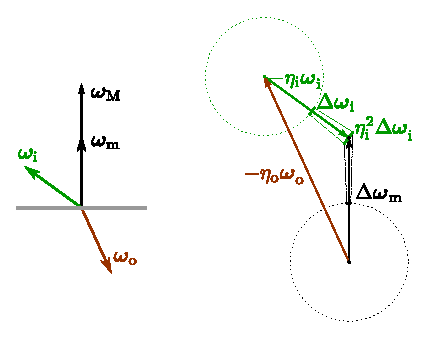
\includegraphics[width=0.6\linewidth]{Pictures/chap08/GeometryForIdealRefraction.eps}
    \caption{镜面折射中的角度扰动关系和相应雅可比矩阵行列式绝对值的计算。}
    \label{fig:08ex01-GeometryForIdealRefraction}
\end{figure}

如\reffig{08ex01-GeometryForIdealRefraction}所示,和上节类似,
我们根据立体角的定义以及上式的几何含义画出扰动时的情况:
当${\bm\omega}_{\mathrm{i}}$发生扰动$\Delta{\bm\omega}_{\mathrm{i}}$时,
向量$-\eta_{\mathrm{i}}{\bm\omega}_{\mathrm{i}}$末端扰动面积
为$\eta^2_{\mathrm{i}}\Delta{\bm\omega}_{\mathrm{i}}$,
用它在${\bm\omega}_{\mathrm{m}}$方向的投影面积
除以${\bm\omega}_{\mathrm{M}}$模的平方即可得到对应的立体角扰动量,
取绝对值后得
\begin{align}
    \left\lVert\frac{\partial{\bm\omega}_{\mathrm{m}}}{\partial{\bm\omega}_{\mathrm{i}}}\right\rVert
    =&\lim\limits_{\Delta{\bm\omega}_{\mathrm{i}}\to0}\frac{|\Delta{\bm\omega}_{\mathrm{m}}|}{|\Delta{\bm\omega}_{\mathrm{i}}|}
    =\frac{|\eta^2_{\mathrm{i}}\Delta{\bm\omega}_{\mathrm{i}}|
    \cdot|{\bm\omega}_{\mathrm{i}}\cdot{\bm\omega}_{\mathrm{m}}|}
    {|\Delta{\bm\omega}_{\mathrm{i}}|\cdot|{\bm\omega}_{\mathrm{M}}|^2}\nonumber\\
    =&\frac{\eta^2_{\mathrm{i}}\cdot|{\bm\omega}_{\mathrm{i}}\cdot{\bm\omega}_{\mathrm{m}}|}
    {(\eta_{\mathrm{i}}({\bm\omega}_{\mathrm{i}}\cdot{\bm\omega}_{\mathrm{m}})
    +\eta_{\mathrm{o}}({\bm\omega}_{\mathrm{o}}\cdot{\bm\omega}_{\mathrm{m}}))^2}\nonumber\\
    =&\frac{|{\bm\omega}_{\mathrm{i}}\cdot{\bm\omega}_{\mathrm{m}}|}
    {\displaystyle(({\bm\omega}_{\mathrm{i}}\cdot{\bm\omega}_{\mathrm{m}})
    +\frac{1}{\eta}({\bm\omega}_{\mathrm{o}}\cdot{\bm\omega}_{\mathrm{m}}))^2}\, .
\end{align}
将上式和\refeq{08ex01-DeltaChangeVar}代入\refeq{08ex01-FresnelBRDFMicrofacet},
并注意对于折射的情况应该把$F_{\mathcal{M}}({\bm\omega}_{\mathrm{h}},{\bm\omega}_{\mathrm{o}})$替换
为$(1-F_{\mathcal{M}}({\bm\omega}_{\mathrm{h}},{\bm\omega}_{\mathrm{o}}))$,即得微曲面上的微观BTDF为
\begin{align}
    f_{\mathcal{M}}({\bm\omega}_{\mathrm{h}},{\bm\omega}_{\mathrm{o}},{\bm\omega}_{\mathrm{i}})
    =\frac{(1-F_{\mathcal{M}}({\bm\omega}_{\mathrm{h}},{\bm\omega}_{\mathrm{o}}))
    \delta_{{\bm\omega}_{\mathrm{m}}}({\bm\omega}_{\mathrm{h}})
    |{\bm\omega}_{\mathrm{i}}\cdot{\bm\omega}_{\mathrm{m}}|}
    {|{\bm\omega}_{\mathrm{h}}\cdot{\bm\omega}_{\mathrm{i}}|
    \displaystyle(({\bm\omega}_{\mathrm{i}}\cdot{\bm\omega}_{\mathrm{m}})
    +\frac{1}{\eta}({\bm\omega}_{\mathrm{o}}\cdot{\bm\omega}_{\mathrm{m}}))^2}\, .
\end{align}

将上式代入\refeq{08ex01-MacroBRDFG2}且把$\max$项替换为取绝对值。
注意被积项中因为存在狄拉克$\delta$分布,所以其只在完美镜面折射成立时,
即${\bm\omega}_{\mathrm{h}}={\bm\omega}_{\mathrm{m}}$时才可能取非零值。
所以最终镜面微面模型的BTDF是
\begin{align}\label{eq:08ex01-BTDFMicrofacetFinal}
    f_{\mathrm{t}}({\bm\omega}_{\mathrm{o}},{\bm\omega}_{\mathrm{i}})
     & =\frac{1}{|{\bm\omega}_{\mathrm{g}}\cdot{\bm\omega}_{\mathrm{i}}||{\bm\omega}_{\mathrm{g}}\cdot{\bm\omega}_{\mathrm{o}}|}
    \int\limits_{\varOmega}\frac{(1-F_{\mathcal{M}}({\bm\omega}_{\mathrm{h}},{\bm\omega}_{\mathrm{o}}))
    \delta_{{\bm\omega}_{\mathrm{m}}}({\bm\omega}_{\mathrm{h}})
    |{\bm\omega}_{\mathrm{i}}\cdot{\bm\omega}_{\mathrm{m}}|}
    {|{\bm\omega}_{\mathrm{h}}\cdot{\bm\omega}_{\mathrm{i}}|
    \displaystyle(({\bm\omega}_{\mathrm{i}}\cdot{\bm\omega}_{\mathrm{m}})
    +\frac{1}{\eta}({\bm\omega}_{\mathrm{o}}\cdot{\bm\omega}_{\mathrm{m}}))^2}\nonumber\\
     & \qquad\qquad\cdot|{\bm\omega}_{\mathrm{h}}\cdot{\bm\omega}_{\mathrm{i}}|
     |{\bm\omega}_{\mathrm{h}}\cdot{\bm\omega}_{\mathrm{o}}|
    G_2({\bm\omega}_{\mathrm{h}},{\bm\omega}_{\mathrm{o}},{\bm\omega}_{\mathrm{i}})
    D({\bm\omega}_{\mathrm{h}})\mathrm{d}{\bm\omega}_{\mathrm{h}}\nonumber\\
     & =\frac{D({\bm\omega}_{\mathrm{m}})G_2({\bm\omega}_{\mathrm{m}},{\bm\omega}_{\mathrm{o}},{\bm\omega}_{\mathrm{i}})
        (1-F_{\mathcal{M}}({\bm\omega}_{\mathrm{m}},{\bm\omega}_{\mathrm{o}}))
        |{\bm\omega}_{\mathrm{m}}\cdot{\bm\omega}_{\mathrm{i}}||{\bm\omega}_{\mathrm{m}}\cdot{\bm\omega}_{\mathrm{o}}|}
     {|{\bm\omega}_{\mathrm{g}}\cdot{\bm\omega}_{\mathrm{i}}||{\bm\omega}_{\mathrm{g}}\cdot{\bm\omega}_{\mathrm{o}}|
     \displaystyle(({\bm\omega}_{\mathrm{i}}\cdot{\bm\omega}_{\mathrm{m}})
    +\frac{1}{\eta}({\bm\omega}_{\mathrm{o}}\cdot{\bm\omega}_{\mathrm{m}}))^2}\, .
\end{align}

\subsection{微面模型BRDF的规范化测试}\label{sub:微面模型BRDF的规范化测试}
本节继承上节的记号。假设某材质不吸收任何入射辐射能量,
且菲涅耳反射率$F_{\mathcal{M}}({\bm\omega}_{\mathrm{m}},{\bm\omega}_{\mathrm{o}})$恒为1,
也即完全不透射任何光线,则入射的能量会被无损地反射回去。
此时对应的BRDF应该满足以下规范化约束:
\begin{align}\label{eq:08ex-01-WhiteFurnaceTest}
    \forall {\bm\omega}_{\mathrm{o}}: \quad\int\limits_{{\varOmega}_{\mathrm{i}}}
    f_{\mathrm{r}}({\bm\omega}_{\mathrm{o}},{\bm\omega}_{\mathrm{i}})
    |{\bm\omega}_{\mathrm{g}}\cdot{\bm\omega}_{\mathrm{i}}|\mathrm{d}{\bm\omega}_{\mathrm{i}}=1\, ,
\end{align}
上式称作\keyindex{白炉测试}{White Furnace Test}{}等式。
该式意味着,对于这样的材质,由出射光线反推回去的入射光线,
会在表面上反射一次或多次,最终全部离开表面,且无能量损失。

然而常见的可解析表达的BRDF都没有考虑多次反射的情况,
这些多次反射的光线都被遮挡函数滤除了,
所以此类BRDF在完美镜面微面模型上作参数化时都不满足白炉测试等式。
因此我们换个角度来分析——我们考虑光线刚发生第一次反射之后、离开曲面之前的情况,
即把掩模遮挡函数替换为只有掩模函数函数
(令$G_2({\bm\omega}_{\mathrm{m}},{\bm\omega}_{\mathrm{o}},{\bm\omega}_{\mathrm{i}})
    =G_1({\bm\omega}_{\mathrm{m}},{\bm\omega}_{\mathrm{o}})$),
则规范化约束应重新成立。此时来自\refeq{08ex01-BRDFMicrofacetFinal}的BRDF变为
\begin{align}
    f_{\mathrm{r}}({\bm\omega}_{\mathrm{o}},{\bm\omega}_{\mathrm{i}})
    =\frac{G_1({\bm\omega}_{\mathrm{m}},{\bm\omega}_{\mathrm{o}})D({\bm\omega}_{\mathrm{m}})}
    {4|{\bm\omega}_{\mathrm{g}}\cdot{\bm\omega}_{\mathrm{i}}||{\bm\omega}_{\mathrm{g}}\cdot{\bm\omega}_{\mathrm{o}}|}\, .
\end{align}
将其代入白炉测试\refeq{08ex-01-WhiteFurnaceTest},
便得到\keyindex{弱白炉测试}{Weak White Furnace Test}{White Furnace Test白炉测试}等式:
\begin{align}\label{eq:08ex01-WeakWhiteFurnaceTest}
    \forall {\bm\omega}_{\mathrm{o}}: \quad\int\limits_{{\varOmega}_{\mathrm{i}}}
    \frac{G_1({\bm\omega}_{\mathrm{m}},{\bm\omega}_{\mathrm{o}})D({\bm\omega}_{\mathrm{m}})}
    {4|{\bm\omega}_{\mathrm{g}}\cdot{\bm\omega}_{\mathrm{o}}|}\mathrm{d}{\bm\omega}_{\mathrm{i}}=1\, .
\end{align}
容易看出,上式的成立其实并不依赖菲涅耳反射率恒为1。
它给出了镜面微面模型对$G_1$的又一重要约束。
需要说明的是,弱白炉测试丢弃遮挡函数只是为了
提供一个便捷的方法来验证BRDF的物理合理性,
并不是说BRDF在实际使用中也应丢弃遮挡函数(\reffig{08ex01-CompleteWhiteFurnaceTest})。
\begin{figure}[htbp]
    \centering
    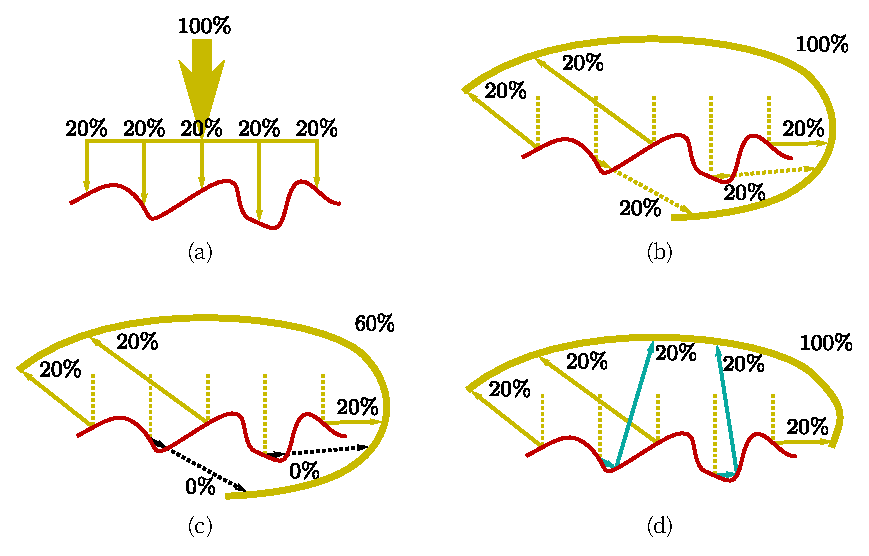
\includegraphics[width=\linewidth]{Pictures/chap08/CompleteWhiteFurnaceTest.eps}
    \caption{基于镜面微面模型的BRDF的规范性:反推光路时,(a)令出射光线照在微面上;
    (b)若光线从不被遮挡(也即只考虑首次反射),则能量总量不变,反射光线满足规范性;
    (c)若BRDF剔除了被遮挡的光线(黑虚线),则能成功反射的能量变少,规范性被打破;
    (d)但实际上被遮挡的光线会多反射几次后射出(蓝绿线),完整的BRDF把这种多次散射的情况纳入考虑后,规范性应重新成立。}
    \label{fig:08ex01-CompleteWhiteFurnaceTest}
\end{figure}

在实践中,我们经常会面临这样一个问题:
某个基于镜面微面模型的BRDF是“基于物理的”吗?
回顾这四个小节的内容,我们虽然不能正面给出答案,
但却可以给出一些有效的验证方法——
如果这个BRDF没有同时满足以下四个规范化约束,那它必然不是“基于物理的”:
\begin{enumerate}
    \item 微面分布函数$D({\bm\omega}_{\mathrm{h}})$满足\refeq{08ex01-McrofacetDistributionNormalization};
    \item 掩模函数$G_1$满足\refeq{08ex01-CosThetaO};
    \item 可见法线分布$D_{{\bm\omega}_{\mathrm{o}}}({\bm\omega}_{\mathrm{h}})$满足\refeq{08ex01-VisibleDistributionNormalization};
    \item 弱白炉测试\refeq{08ex01-WeakWhiteFurnaceTest}成立。
\end{enumerate}
但这并不意味着不能使用那些无法同时满足上述约束的非“基于物理的”BRDF,
完全可以根据实际需要做出相应选择,何况以上结论考虑的还是最简单的情况。
多次反射、多层材料、存在衍射等更复杂的情况还需进一步探索。

\subsection{常见掩模函数的分析}\label{sub:常见掩模函数的分析}
本节继承上节的记号。本节将分析Smith和V形槽两种微面结构,推导它们的掩模函数并讨论其性质。
其他没有相应微面结构因而并非基于物理的常见掩模函数也会有所讨论。

\subsubsection*{Smith微面}
在Smith微面的构造中,它假设微面是非\keyindex{自相关的}{autocorrelated}{}——
不论微面上的一点和它的临近点有多近,它们的高度(或法线)之间是没有相关性的。
这意味着微面上一点的高度和法线是随机变量,整个曲面是微面的随机集合,而不是通常的连续曲面。
另一方面,法线${\bm\omega}_{\mathrm{h}}$某种意义上是微面的\emph{局部}属性,
而对该点产生遮挡的别处微面则是一种\emph{远距}属性(但仍是微观尺度上的)。
在非自相关假设下,局部属性和远距属性应是独立的,所以掩模函数$G_1$可以拆分为两部分:
\begin{align}\label{eq:08ex01-SeparableMaskingFunction}
    G_1({\bm\omega}_{\mathrm{h}},{\bm\omega}_{\mathrm{o}})
    =G_1^{\mathrm{l}}({\bm\omega}_{\mathrm{h}},{\bm\omega}_{\mathrm{o}})
    G_1^{\mathrm{d}}({\bm\omega}_{\mathrm{o}})\, ,
\end{align}
其中局部掩模函数$G_1^{\mathrm{l}}$就简单地滤除背向的微面:
\begin{align}\label{eq:08ex01-LocalMaskFunction}
    G_1^{\mathrm{l}}({\bm\omega}_{\mathrm{h}},{\bm\omega}_{\mathrm{o}})
    =\chi({\bm\omega}_{\mathrm{h}}\cdot{\bm\omega}_{\mathrm{o}})\, .
\end{align}
这里示性函数$\chi$的定义为
\begin{align}
    \chi(a)=\left\{\begin{array}{l}
        1,\quad\text{若}a>0, \\
        0,\quad\text{其他}.
    \end{array}\right.
\end{align}
而远距掩模函数$G_1^{\mathrm{d}}({\bm\omega}_{\mathrm{o}})$表示
被远处微面遮挡的概率,它独立于局部法线${\bm\omega}_{\mathrm{h}}$.

将\refeq{08ex01-SeparableMaskingFunction}和\refeq{08ex01-LocalMaskFunction}
代入\refeq{08ex01-CosThetaO},可得
\begin{align}
    \cos\theta_{\mathrm{o}}
     & =\int\limits_{\varOmega}G_1({\bm\omega}_{\mathrm{h}},{\bm\omega}_{\mathrm{o}})
    \max({\bm\omega}_{\mathrm{h}}\cdot{\bm\omega}_{\mathrm{o}},0)
    D({\bm\omega}_{\mathrm{h}})\mathrm{d}{\bm\omega}_{\mathrm{h}}\nonumber                         \\
     & =\int\limits_{\varOmega}G_1^{\mathrm{l}}({\bm\omega}_{\mathrm{h}},{\bm\omega}_{\mathrm{o}})
    G_1^{\mathrm{d}}({\bm\omega}_{\mathrm{o}})
    \max({\bm\omega}_{\mathrm{h}}\cdot{\bm\omega}_{\mathrm{o}},0)
    D({\bm\omega}_{\mathrm{h}})\mathrm{d}{\bm\omega}_{\mathrm{h}}\nonumber                         \\
     & =\int\limits_{\varOmega}\chi({\bm\omega}_{\mathrm{h}}\cdot{\bm\omega}_{\mathrm{o}})
    G_1^{\mathrm{d}}({\bm\omega}_{\mathrm{o}})
    \max({\bm\omega}_{\mathrm{h}}\cdot{\bm\omega}_{\mathrm{o}},0)
    D({\bm\omega}_{\mathrm{h}})\mathrm{d}{\bm\omega}_{\mathrm{h}}\nonumber                         \\
     & =G_1^{\mathrm{d}}({\bm\omega}_{\mathrm{o}})\int\limits_{\varOmega}
    \max({\bm\omega}_{\mathrm{h}}\cdot{\bm\omega}_{\mathrm{o}},0)
    D({\bm\omega}_{\mathrm{h}})\mathrm{d}{\bm\omega}_{\mathrm{h}}\, .
\end{align}
于是
\begin{align}\label{eq:08-ex01-g1_distance}
    G_1^{\mathrm{d}}({\bm\omega}_{\mathrm{o}})
    =\frac{\cos\theta_{\mathrm{o}}}
    {\displaystyle\int\limits_{\varOmega}\max({\bm\omega}_{\mathrm{h}}\cdot{\bm\omega}_{\mathrm{o}},0)
    D({\bm\omega}_{\mathrm{h}})\mathrm{d}{\bm\omega}_{\mathrm{h}}}\, .
\end{align}
所以完整的掩模函数为
\begin{align}\label{eq:08-ex01-masking-g1-int}
    G_1({\bm\omega}_{\mathrm{h}},{\bm\omega}_{\mathrm{o}})
    =\frac{\chi({\bm\omega}_{\mathrm{h}}\cdot{\bm\omega}_{\mathrm{o}})\cos\theta_{\mathrm{o}}}
    {\displaystyle\int\limits_{\varOmega}\max({\bm\omega}\cdot{\bm\omega}_{\mathrm{o}},0)
        D({\bm\omega})\mathrm{d}{\bm\omega}}\, .
\end{align}
这恰是\citet{10.1145/344779.344814}在法线和遮挡独立性假设下
得到的掩模函数的精确积分形式。然而其中的积分是在法线分布空间中进行的,
计算起来并不方便。我们可以将其积分域转化到斜率分布空间以简化它,下面给出具体推导。

对于曲面上某处的法线${\bm\omega}_{\mathrm{h}}$,
设它在直角坐标系下和球面坐标系下具体的分量为
\begin{align}
    {\bm\omega}_{\mathrm{h}}=(x_{\mathrm{h}},y_{\mathrm{h}},z_{\mathrm{h}})
    =(\sin\theta\cos\varphi,\sin\theta\sin\varphi,\cos\theta)\, ,
\end{align}
其中$\theta$为天顶角(即${\bm\omega}_{\mathrm{h}}\cdot{\bm\omega}_{\mathrm{g}}=\cos\theta$),
$\varphi$为方位角
\sidenote{参见\reffig{5.ex01}。};则该处附近的面元可以近似为以下平面
\begin{align}
    x_{\mathrm{h}}x+y_{\mathrm{h}}y+z_{\mathrm{h}}z=C\, .
\end{align}
其中$C$为某个常量,于是有
\begin{align}
    z=\left(-\frac{x_{\mathrm{h}}}{z_{\mathrm{h}}},
    -\frac{y_{\mathrm{h}}}{z_{\mathrm{h}}}\right)\cdot(x,y)+C\, ,
\end{align}
我们由此定义
\begin{align}\label{eq:08-ex01-slope-of-surface}
    {\bm s}({\bm\omega}_{\mathrm{h}})=(x_s,y_s)
    =\left(-\frac{x_{\mathrm{h}}}{z_{\mathrm{h}}},
    -\frac{y_{\mathrm{h}}}{z_{\mathrm{h}}}\right)
    =-\tan\theta(\cos\varphi,\sin\varphi)
\end{align}
为曲面在该处的斜率
\sidenote{原文slope,这里作者想表达的是$z$对$x$和$y$的偏导数,
    它和二维直角坐标系下直线斜率的形式很像,所以借用这个称呼。}。
反之,也可以根据斜率求出相应法线为
\sidenote{注意到${\bm s}({\bm\omega}_{\mathrm{h}})={\bm s}(-{\bm\omega}_{\mathrm{h}})$,
所以这里也可以是反向的结果,我们只是取其中一个。}
\begin{align}\label{eq:08-ex01-normals-by-slope}
    {\bm\omega}_{\mathrm{h}}=\frac{1}{\sqrt{x_s^2+y_s^2+1}}(-x_s,-y_s,1)\, .
\end{align}

接下来我们考虑斜率分布$P_{xy}({\bm s})$与法线分布
(即微面分布函数)$D({\bm\omega}_{\mathrm{h}})$之间的关系。
法线分布方面,根据三维球面坐标转换
公式\sidenote{见第\refsec{球体}。},有
\begin{align}\label{eq:08-ex01-D_sphere}
    D({\bm\omega}_{\mathrm{h}})\mathrm{d}{\bm\omega}_{\mathrm{h}}
    =D({\bm\omega}_{\mathrm{h}})\sin\theta\mathrm{d}\theta\mathrm{d}\varphi\, .
\end{align}
斜率分布方面,其积分也有换元关系
\sidenote{这是微积分中常用的换元方法,此处我们不探究其使用条件,读者可参考相关教材。}
\begin{align}\label{eq:08-ex01-Pxy-Jacobian}
    P_{xy}(x_s,y_s)\mathrm{d}x_s\mathrm{d}y_s
    =P_{xy}(x_s,y_s)|J|\mathrm{d}\theta\mathrm{d}\varphi\, ,
\end{align}
其中$J$为$(x_s,y_s)$对参数$(\theta,\varphi)$的雅可比矩阵
\begin{align}
    J=\displaystyle\frac{\partial(x_s,y_s)}{\partial(\theta,\varphi)}
    =\displaystyle\left[\begin{array}{cc}
            \displaystyle\frac{\partial x_s}{\partial \theta} &
            \displaystyle\frac{\partial x_s}{\partial \varphi}  \\
            \displaystyle\frac{\partial y_s}{\partial \theta} &
            \displaystyle\frac{\partial y_s}{\partial \varphi}
        \end{array}\right]
    =\displaystyle\left[\begin{array}{rr}
            \displaystyle -\frac{\cos\varphi}{\cos^2\theta} &
            \displaystyle \tan\theta\sin\varphi               \\
            \displaystyle -\frac{\sin\varphi}{\cos^2\theta} &
            \displaystyle -\tan\theta\cos\varphi
        \end{array}\right]\, ,
\end{align}
于是雅可比行列式为
\begin{align}\label{eq:08-ex01-Jacobian-slope-normals}
    |J|=\left(\frac{\partial x_s}{\partial \theta}\frac{\partial y_s}{\partial \varphi}
    -\frac{\partial x_s}{\partial \varphi}\frac{\partial y_s}{\partial \theta}\right)
    =\frac{\tan\theta}{\cos^2\theta}\, .
\end{align}
注意到$P_{xy}({\bm s})$应满足规范化约束,
即它在$x_s\in(-\infty,+\infty),y_s\in(-\infty,+\infty)$范围内非负,且有
\begin{align}\label{eq:08-ex01-normal-of-P2D}
    \int_{-\infty}^{+\infty}\int_{-\infty}^{+\infty}
    P_{xy}(x_s,y_s)\mathrm{d}x_s\mathrm{d}y_s=1\, .
\end{align}
将上式和\refeq{08ex01-McrofacetDistributionNormalization}比对,可得
\begin{align}\label{eq:08-ex01-P2D}
    P_{xy}(x_s,y_s)\mathrm{d}x_s\mathrm{d}y_s=
    D({\bm\omega}_{\mathrm{h}})\cos\theta\mathrm{d}{\bm\omega}_{\mathrm{h}}\, .
\end{align}
联立\refeq{08-ex01-D_sphere}、\refeq{08-ex01-Pxy-Jacobian}和\refeq{08-ex01-P2D}可得
\begin{align}
    P_{xy}(x_s,y_s)|J|\mathrm{d}\theta\mathrm{d}\varphi
    =D({\bm\omega}_{\mathrm{h}})\sin\theta\cos\theta\mathrm{d}\theta\mathrm{d}\varphi\, ,
\end{align}
代入\refeq{08-ex01-Jacobian-slope-normals}后可知斜率分布与法线分布的关系为
\begin{align}\label{eq:08-ex01-relation-P2D-McrofacetDistribution}
    P_{xy}(x_s,y_s)=\frac{1}{|J|}D({\bm\omega}_{\mathrm{h}})\sin\theta\cos\theta
    =D({\bm\omega}_{\mathrm{h}})\cos^4\theta\, .
\end{align}

只有$P_{xy}(x_s,y_s)$还不足以推导出掩模遮挡函数。
我们可以把微曲面$\mathcal{M}$看作是在光滑的宏曲面$\mathcal{G}$上
通过平稳的随机过程叠加上或正或负的高度波动得到的。如\reffig{08ex01-G1Geometry}所示,
我们继续分析一个微观区域:仍把宏曲面视作平面,也即$z=0$,宏曲面法线为${\bm\omega}_{\mathrm{g}}=(0,0,1)$。
而微曲面上每一点在$Z$方向到宏曲面上的高度$h$(包含正负号)由连续概率分布$P_H(h)$描述,
且通常$P_H(h)$均值为零。同时我们写出光线出射方向${\bm\omega}_{\mathrm{o}}$的球坐标表示:
\begin{align}
    {\bm\omega}_{\mathrm{o}}=(\sin\theta_{\mathrm{o}}\cos\varphi_{\mathrm{o}},\sin\theta_{\mathrm{o}}\sin\varphi_{\mathrm{o}},\cos\theta_{\mathrm{o}})\, .
\end{align}
其中出射角$\theta_{\mathrm{o}}$即${\bm\omega}_{\mathrm{o}}$与${\bm\omega}_{\mathrm{g}}$的夹角。

接下来我们考虑这样一个问题:在微曲面$\mathcal{M}$上随机取一点$A$,
则点$A$具有高度$h_A$,且该点处的微面斜率$(x_s,y_s)$取值为$(u_A,v_A)$,
还能从${\bm\omega}_{\mathrm{o}}$方向可见的概率是多少?

我们把这个概率记作$W(h_A,u_A,v_A,{\bm\omega}_{\mathrm{o}})$.
为了方便考虑该问题,我们在由${\bm\omega}_{\mathrm{o}}$和${\bm\omega}_{\mathrm{g}}$确定的平面
(以下简称“截平面”)内推导:在如\reffig{08ex01-G1Geometry}所示直角坐标系下,
我们把原点$O$取在点$A$正下方的宏曲面上,把$OA$定为纵轴$Z$,${\bm\omega}_{\mathrm{g}}$和$Z$轴同向;
横轴$T$垂直于纵轴$Z$且与${\bm\omega}_{\mathrm{o}}$、${\bm\omega}_{\mathrm{g}}$共面(也即在截平面内),
并和${\bm\omega}_{\mathrm{o}}$朝着同一边。
这样我们就能借鉴之前的光线参数化表示法——微曲面上任意一点的位置都可以
用它在宏曲面(也即横轴$T$)上的投影坐标$t$来表示。
此外,我们在图示中考虑的出射方向大致向右,所以不失一般性,我们假定只有点$A$右边的微曲面才有可能挡住出射光线。
所以$W(h_A,u_A,v_A,{\bm\omega}_{\mathrm{o}})$就是点$A$右侧的微面不会与出射光线相交的概率。

为了简化后文记号,我们以$A$来代替$h_A,u_A,v_A$这整组关于点$A$的变量,
把$W(h_A,u_A,v_A,{\bm\omega}_{\mathrm{o}})$简记为$W(A,{\bm\omega}_{\mathrm{o}})$,
并进一步定义$W(A,{\bm\omega}_{\mathrm{o}},t)$为区间$[0,t]$内的微面都不与光线相交的概率,于是有
\begin{align}\label{eq:08ex01-W-definition}
    W(A,{\bm\omega}_{\mathrm{o}})=\lim\limits_{t\to +\infty}W(A,{\bm\omega}_{\mathrm{o}},t)\, .
\end{align}

根据$W(A,{\bm\omega}_{\mathrm{o}},t)$的定义,它应当满足如下微分性质:
\begin{align}\label{eq:08ex01-VisiblePointProbability}
    W(A,{\bm\omega}_{\mathrm{o}},t+\Delta t)
    =W(A,{\bm\omega}_{\mathrm{o}},t)
    Q(\Delta t|A,{\bm\omega}_{\mathrm{o}},t)\, ,
\end{align}
其中$Q(\Delta t|A,{\bm\omega}_{\mathrm{o}},t)$是微面与光线没有
在区间$[0,t]$内相交的前提下,在极小区间$[t,t+\Delta t]$内
(对应图中微曲面上$C$、$D$两点之间)也不相交的条件概率。
进一步略去符号$A$和${\bm\omega}_{\mathrm{o}}$,我们反过来用$g(t)\Delta t$表示
在区间$[t,t+\Delta t]$内要发生相交(并设交点为$B$)的条件概率
(意味着$g(t)$本身是个概率密度函数),即
\begin{align}
    Q(\Delta t|A,{\bm\omega}_{\mathrm{o}},t)=1-g(t)\Delta t\, ,
\end{align}
代回\refeq{08ex01-VisiblePointProbability},得到
\begin{align}
    W(t+\Delta t)=W(t)(1-g(t)\Delta t)\, .
\end{align}
利用上式取极限,可得微分方程
\begin{align}
    \frac{\mathrm{d}}{\mathrm{d}t}W(t)=\lim\limits_{\Delta t\to 0}\frac{W(t+\Delta t)-W(t)}{\Delta t}=-W(t)g(t)\, ,
\end{align}
并求得解为
\begin{align}\label{eq:08ex01-WtSolution}
    W(t)=W(0)\exp\left(-\int_{0}^{t}g(\tau)\mathrm{d}\tau\right)\, .
\end{align}
其中$\tau$为临时积分变量。

在关注$W(0)$的取值前,我们先插入点$A$的斜率问题。
前面已经设了点$A$处的微面斜率在$x$和$y$方向的取值为$(u_A,v_A)$,
那微曲面被截平面截取后,在被截出的曲线上点$A$处的一维斜率$q_A$
(也即纵轴$Z$方向的高度相对于横轴$T$方向的变化率)是多少?
显然就是微面在出射方向上的方向导数
\begin{align}
    q_A=u_A\cos\varphi_{\mathrm{o}}+v_A\sin\varphi_{\mathrm{o}}\, .
\end{align}
更一般地,把截平面内微曲面上任意一点的一维斜率$q$满足的概率分布记作$P_s(q)$,
那么$P_s(q)$就是二维斜率分布$P_{xy}(x_s,y_s)$积分坍缩到截平面内的结果:
\begin{align}
    P_s(q)=\int_{-\infty}^{+\infty}P_{xy}(q\cos\varphi_{\mathrm{o}}-p\sin\varphi_{\mathrm{o}},
    q\sin\varphi_{\mathrm{o}}+p\cos\varphi_{\mathrm{o}})\mathrm{d}p\, ,
\end{align}
其中$p$为临时积分变量。后文将会介绍到,$P_{xy}(x_s,y_s)$常常满足
各向同性形状不变性,也即意味着$\varphi_{\mathrm{o}}$取任意值
都不改变上式$P_s(q)$的结果。所以不妨设$\varphi_{\mathrm{o}}=0$,
此时$P_s(q)$就是$P_{xy}(x_s,y_s)$的边缘分布$P_x(x_s)$:
\begin{align}\label{eq:08-ex01-condition-1d-slope}
    P_s(q)=P_x(q)=\int_{-\infty}^{+\infty}P_{xy}(q,y_s)\mathrm{d}y_s\, .
\end{align}

回到\refeq{08ex01-WtSolution}中,根据定义,$W(0)$应该这样取值:
若点$A$的一维斜率$q_A$高于光线的斜率$\mu=\cot\theta_{\mathrm{o}}$,
则光线立即被遮挡,该取值0,否则该取1,于是
\begin{align}
    W(0)=\chi(\mu-q_A)\, ,
\end{align}
所以有
\begin{align}\label{eq:08ex01-Wt-gt-int}
    W(t)=\chi(\mu-q_A)\exp\left(-\int_{0}^{t}g(\tau)\mathrm{d}\tau\right)\, .
\end{align}

\begin{figure}[htbp]
    \centering
    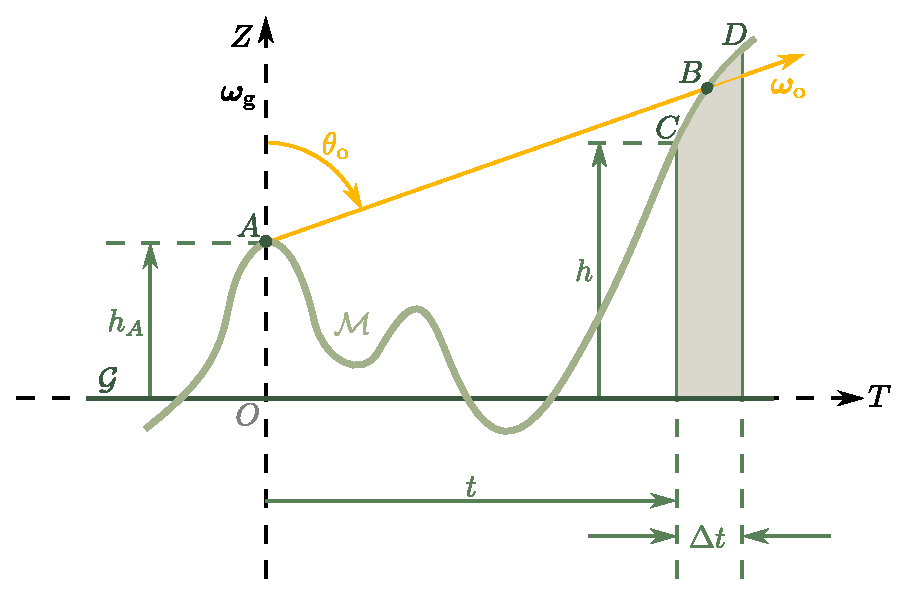
\includegraphics[width=0.8\linewidth]{Pictures/chap08/GeometryForSmithShadowingMasking.eps}
    \caption{求微曲面上点$A$能从${\bm\omega}_{\mathrm{o}}$方向观察到的概率,
    可以先求对应光线在极小区间$[t,t+\Delta t]$内与微曲面相交的条件概率,再作转化。}
    \label{fig:08ex01-G1Geometry}
\end{figure}

接下来的关键是怎么求出上式关于$g(t)$的积分。
为了避免去考虑区间内微曲面上无穷个点的相关性,
我们把这个问题简化近似为:在点$A$发出的光线没有被$t$之前的微面遮挡的条件下,
光线在区间$[t,t+\Delta t]$内会被遮挡的条件概率。
先考虑区间起点:设$t$处的微曲面(也即点$C$)的高度为$h$,一维斜率为$q$,
显然只要微曲面高度$h$低于光线高度$h_A+\mu t$即可,斜率不限:
\begin{align}
    h<h_A+\mu t\, ,
\end{align}
我们把这一事件记作$X$,算出相应的概率为
\begin{align}
    P(X)=\int_{-\infty}^{+\infty}\int_{-\infty}^{h_A+\mu t}
    P_{\mathcal{M}}(h,q|A,t)\mathrm{d}h\mathrm{d}q\, ,
\end{align}
其中$P_{\mathcal{M}}(h,q|A,t)$是给定点$A$和区间位置$t$的前提下,
微曲面上$t$处的高度$h$和一维斜率$q$的联合概率密度函数。

接着考虑区间终点:要发生遮挡,则光线离开区间时应在微曲面之下,
即意味着$t+\Delta t$处(也即点$D$)的微曲面高度应高于光线高度。
因为区间极小,我们近似认为整个区间内微曲面足够平滑,各点一维斜率仍为$q$,于是有
\begin{align}
    h+q\Delta t>h_A+\mu(t+\Delta t)\, ,
\end{align}
整理得
\begin{align}
    h>h_A+\mu t-(q-\mu)\Delta t\, ,
\end{align}
我们把上述条件成立记作事件$Y$。
注意当事件$X$和$Y$同时发生时,还可推出$q>\mu$.
所以事件$X$和$Y$同时发生的概率为
\begin{align}
    P(X,Y)=\int_{\mu}^{+\infty}\int_{h_A+\mu t-(q-\mu)\Delta t}^{h_A+\mu t}
    P_{\mathcal{M}}(h,q|A,t)\mathrm{d}h\mathrm{d}q\, .
\end{align}
通常我们假设高度$h$和一维斜率$q$作为随机变量是相互独立的,再加上非自相关的假设,于是有
\begin{align}
    P_{\mathcal{M}}(h,q|A,t)=P_H(h)P_s(q)\, .
\end{align}
而$g(t)\Delta t$就是事件$Y$对事件$X$的条件概率
\begin{align}
    g(t)\Delta t=P(Y|X)=\frac{P(X,Y)}{P(X)}\, .
\end{align}
利用中值定理,整理化简得
\begin{align}\label{eq:08ex01-gt-expression}
    g(t)=&\lim\limits_{\Delta t\to 0}\frac{P(X,Y)}{\Delta tP(X)}
    =\lim\limits_{\Delta t\to 0}\frac{\displaystyle\int_{\mu}^{+\infty}\int_{h_A+\mu t-(q-\mu)\Delta t}^{h_A+\mu t}
    P_{\mathcal{M}}(h,q|A,t)\mathrm{d}h\mathrm{d}q}{\Delta t\displaystyle\int_{-\infty}^{+\infty}
    \int_{-\infty}^{h_A+\mu t}P_{\mathcal{M}}(h,q|A,t)\mathrm{d}h\mathrm{d}q}\nonumber\\
    =&\frac{\displaystyle\int_{\mu}^{+\infty}(q-\mu)P_s(q)\lim\limits_{\Delta t\to 0}
    \left(\frac{1}{(q-\mu)\Delta t}\int_{h_A+\mu t-(q-\mu)\Delta t}^{h_A+\mu t}P_H(h)\mathrm{d}h\right)\mathrm{d}q}
    {\displaystyle\int_{-\infty}^{h_A+\mu t}P_H(h)\mathrm{d}h}\nonumber\\
    =&\frac{\displaystyle\int_{\mu}^{+\infty}(q-\mu)P_s(q)P_H(h_A+\mu t)\mathrm{d}q}
    {\displaystyle\int_{-\infty}^{h_A+\mu t}P_H(h)\mathrm{d}h}
    =\Lambda(\mu)\frac{\mu P_H(h_A+\mu t)}{F_H(h_A+\mu t)}\, ,
\end{align}
其中$F_H$是$P_H$相应的累积分布函数
\begin{align}
    F_H(h)=\int_{-\infty}^{h}P_H(\xi)\mathrm{d}\xi\, ,
\end{align}
其中$\xi$为临时积分变量,而$\Lambda(\mu)$则定义为
\begin{align}
    \Lambda(\mu)=\frac{1}{\mu}\int_{\mu}^{+\infty}(q-\mu)P_s(q)\mathrm{d}q\, .
\end{align}
注意到
\begin{align}
    \frac{\partial F_H(h_A+\mu t)}{\partial t}=\mu P_H(h_A+\mu t)\, ,
\end{align}
再联立\refeq{08ex01-W-definition}、\refeq{08ex01-Wt-gt-int}和\refeq{08ex01-gt-expression},得到
\begin{align}
    W(A,{\bm\omega}_{\mathrm{o}})=&\chi(\mu-q_A)\exp\left(-\int_{0}^{+\infty}g(t)\mathrm{d}t\right)\nonumber\\
    =&\chi(\mu-q_A)\exp\left(-\int_{0}^{+\infty}\Lambda(\mu)\frac{\mu P_H(h_A+\mu t)}{F_H(h_A+\mu t)}\mathrm{d}t\right)\nonumber\\
    =&\chi(\mu-q_A)\exp\left(-\Lambda(\mu)\int_{0}^{+\infty}\mathrm{d}\ln F_H(h_A+\mu t)\right)\nonumber\\
    =&\chi(\mu-q_A)\exp\left(-\Lambda(\mu)(\ln 1 - \ln F_H(h_A))\right)\nonumber\\
    =&\chi(\mu-q_A)F_H^{\Lambda(\mu)}(h_A)\, .
\end{align}
我们在被观察点$A$的所有高度$h_A$上积分,并再次利用$F_H$和$P_H$之间的微分关系,
就得到该光线对微曲面上点$A$所有可能的情况的可见概率均值为
\begin{align}\label{eq:08ex01-AverageVisibleProbability}
    W(u_A,v_A,{\bm\omega}_{\mathrm{o}})&=\int_{-\infty}^{+\infty}W(A,{\bm\omega}_{\mathrm{o}})P_H(h_A)\mathrm{d}h_A\nonumber\\
    =&\int_{-\infty}^{+\infty}\chi(\mu-q_A)F_H^{\Lambda(\mu)}(h_A)P_H(h_A)\mathrm{d}h_A\nonumber\\
    =&\chi(\mu-q_A)\int_{-\infty}^{+\infty}F_H^{\Lambda(\mu)}(h_A)\mathrm{d}F_H(h_A)\nonumber\\
    =&\chi(\mu-q_A)\frac{F_H^{1+\Lambda(\mu)}(h_A)}{1+\Lambda(\mu)}\bigg|_{h_A=-\infty}^{+\infty}\nonumber\\
    =&\frac{\chi(\mu-q_A)}{1+\Lambda(\mu)}\, .
\end{align}
考虑到$\chi(\mu-q_A)$就是表示滤除背向光线的意思,
它可以等价替换为$\chi({\bm\omega}_{\mathrm{h}}\cdot{\bm\omega}_{\mathrm{o}})$;
$\Lambda(\mu)$中$\mu$也由${\bm\omega}_{\mathrm{o}}$决定,
可重新记作$\Lambda({\bm\omega}_{\mathrm{o}})$;
而$W(u_A,v_A,{\bm\omega}_{\mathrm{o}})$就是我们想求得的掩模遮挡函数,于是最终得到
\begin{align}\label{eq:08-ex01-Smith-masking-function}
    G_1({\bm\omega}_{\mathrm{h}},{\bm\omega}_{\mathrm{o}})
    =\frac{\chi({\bm\omega}_{\mathrm{h}}\cdot{\bm\omega}_{\mathrm{o}})}
    {1+\Lambda({\bm\omega}_{\mathrm{o}})}\, .
\end{align}
特别地,当$\varphi_{\mathrm{o}}=0$时:
\begin{align}\label{eq:08-ex01-Lambda-function}
    \Lambda({\bm\omega}_{\mathrm{o}})=\frac{1}{\cot\theta_{\mathrm{o}}}
    \int_{\cot\theta_{\mathrm{o}}}^{+\infty}(x_s-\cot\theta_{\mathrm{o}})P_x(x_s)\mathrm{d}x_s\, .
\end{align}

由于前面的推导都是严格等式,没有近似项,这说明在非自相关的假设下,
Smith掩模函数是准确的。此外也有变量代换为主的推导方法,可以得出一样的结果。
在实践中,该模型预测的结果和实测数据非常接近,但仍有偏差,
这是由描述曲面的统计模型(高度和斜率分布函数)和非自相关假设引起的。
现实中的连续曲面往往都有范围很宽的自相关函数。
但\citet{841905}表明忽略自相关性引发的误差仅在观察角度
满足$\tan\theta_{\mathrm{o}}>\frac{\sqrt{2}}{2}\sigma$时
才足够明显($\sigma^2$为斜率的方差),所以通常可以认为
Smith掩模函数可以较为准确地适用于自相关的曲面,
但具有重复性或结构化纹理的材料(例如布料)则不应在建模时忽视这种自相关性。

注意\refeq{08ex01-AverageVisibleProbability}和\refeq{08-ex01-Smith-masking-function}是
在微面的高度上作平均来推导掩模函数它。
因为高度独立于BRDF中的法线,所以我们可以这样作平均。
而且还注意到其结果不依赖特定的高度分布$P_H(h)$.
此外也有对法线作平均的方法,但它对于本文基于几何光学的BRDF来说无关紧要,
而且难以处理,所以此处不再赘述。


\subsubsection*{V形槽微面}
如\reffig{08ex01-V-cavityScatteringModel},V形槽微面模型也是常用模型之一。
它不再是对具有特定法线分布的微面的散射情况进行建模,
而是计算每个独立镜面微面的散射再作平均。每块V形槽都有两个具备对称性的法线,
即${\bm\omega}_{\mathrm{h}}=(x_{\mathrm{h}},y_{\mathrm{h}},z_{\mathrm{h}})$和
${\bm\omega}'_{\mathrm{h}}=(-x_{\mathrm{h}},-y_{\mathrm{h}},z_{\mathrm{h}})$,
它们最后以$\max({\bm\omega}_{\mathrm{h}}\cdot{\bm\omega}_{\mathrm{g}},0)D({\bm\omega}_{\mathrm{h}})$
作为权重合成最终的BRDF。
根据这些特性,我们构造出相应的微面分布函数
\begin{align}\label{eq:08ex01-VCavityScatteringNormalDistribution}
    D({\bm\omega})=\frac{1}{2}\left(
    \frac{\delta_{{\bm\omega}_{\mathrm{h}}}({\bm\omega})}
    {{\bm\omega}_{\mathrm{h}}\cdot{\bm\omega}_{\mathrm{g}}}
    +\frac{\delta_{{\bm\omega}'_{\mathrm{h}}}({\bm\omega})}
    {{\bm\omega}'_{\mathrm{h}}\cdot{\bm\omega}_{\mathrm{g}}}\right)\, .
\end{align}
可以验证\refeq{08ex01-VCavityScatteringNormalDistribution}满足
规范化条件\refeq{08ex01-McrofacetDistributionNormalization}。

\begin{figure}[htbp]
    \centering
    \includegraphics[width=0.8\linewidth]{Pictures/chap08/VCavityScatteringModel.eps}
    \caption{V形槽微面模型。}
    \label{fig:08ex01-V-cavityScatteringModel}
\end{figure}

将\refeq{08ex01-VCavityScatteringNormalDistribution}代入约束条件\refeq{08ex01-CosThetaO},可得
\begin{align}\label{eq:08ex01-V-Cavity-configurations}
    \cos\theta_{\mathrm{o}}=\frac{1}{2}\left(
    G_1({\bm\omega}_{\mathrm{h}},{\bm\omega}_{\mathrm{o}})
    \frac{\max({\bm\omega}_{\mathrm{h}}\cdot{\bm\omega}_{\mathrm{o}},0)}
    {{\bm\omega}_{\mathrm{h}}\cdot{\bm\omega}_{\mathrm{g}}}
    +G_1({\bm\omega}'_{\mathrm{h}},{\bm\omega}_{\mathrm{o}})
    \frac{\max({\bm\omega}'_{\mathrm{h}}\cdot{\bm\omega}_{\mathrm{o}},0)}
    {{\bm\omega}'_{\mathrm{h}}\cdot{\bm\omega}_{\mathrm{g}}}\right)\, .
\end{align}

如\reffig{08ex01-V-cavityScattering-Mask},微面的可见性有两种情况。
一种是其中一个${\bm\omega}'_{\mathrm{h}}$因背向而不可见,
即$G_1({\bm\omega}'_{\mathrm{h}},{\bm\omega}_{\mathrm{o}})=0$,
此时\refeq{08ex01-V-Cavity-configurations}可以简化为
\begin{align}
    \cos\theta_{\mathrm{o}}=\frac{1}{2}G_1({\bm\omega}_{\mathrm{h}},{\bm\omega}_{\mathrm{o}})
    \frac{\max({\bm\omega}_{\mathrm{h}}\cdot{\bm\omega}_{\mathrm{o}},0)}
    {{\bm\omega}_{\mathrm{h}}\cdot{\bm\omega}_{\mathrm{g}}}\, .
\end{align}
由此得到
\begin{align}
    G_1({\bm\omega}_{\mathrm{h}},{\bm\omega}_{\mathrm{o}})
    =\frac{2({\bm\omega}_{\mathrm{h}}\cdot{\bm\omega}_{\mathrm{g}})\cos\theta_{\mathrm{o}}}
    {\max({\bm\omega}_{\mathrm{h}}\cdot{\bm\omega}_{\mathrm{o}},0)}
    =\frac{2({\bm\omega}_{\mathrm{h}}\cdot{\bm\omega}_{\mathrm{g}})
    ({\bm\omega}_{\mathrm{o}}\cdot{\bm\omega}_{\mathrm{g}})}
    {\max({\bm\omega}_{\mathrm{h}}\cdot{\bm\omega}_{\mathrm{o}},0)}\, .
\end{align}

\begin{figure}[htbp]
    \centering
    \includegraphics[width=0.9\linewidth]{Pictures/chap08/VCavityMicrosurfaceMask.eps}
    \caption{V形槽微面模型的掩模。(a)一个面完全不可见,另一个被部分遮挡;
        (b)两个面都完全可见,此时掩模函数值为1.}
    \label{fig:08ex01-V-cavityScattering-Mask}
\end{figure}

另一种情况是${\bm\omega}_{\mathrm{h}}$和${\bm\omega}'_{\mathrm{h}}$均完全可见,
即$G_1({\bm\omega}_{\mathrm{h}},{\bm\omega}_{\mathrm{o}})=G_1({\bm\omega}'_{\mathrm{h}},{\bm\omega}_{\mathrm{o}})=1$.
我们以单个表达式概括上述两种情况:
\begin{align}\label{eq:08ex01-V-Cavity-MaskingFunction}
    G_1({\bm\omega}_{\mathrm{h}},{\bm\omega}_{\mathrm{o}})
    =\min\left(1, \frac{2({\bm\omega}_{\mathrm{h}}\cdot{\bm\omega}_{\mathrm{g}})
    ({\bm\omega}_{\mathrm{o}}\cdot{\bm\omega}_{\mathrm{g}})}
    {\max({\bm\omega}_{\mathrm{h}}\cdot{\bm\omega}_{\mathrm{o}},0)}\right)\, .
\end{align}
这便是\citet{10.1145/357290.357293}所用的著名的V形槽掩模函数。

现在我们验证下\refeq{08ex01-V-Cavity-MaskingFunction}是否满足
可见法线分布的规范化约束即\refeq{08ex01-VisibleDistributionNormalization}。
先将$G_1({\bm\omega}_{\mathrm{h}},{\bm\omega}_{\mathrm{o}})$代入\refeq{08ex01-DistributionOfVisibleNormals}得
\begin{align}
    D_{{\bm\omega}_{\mathrm{o}}}({\bm\omega}_{\mathrm{h}})
    =\min\left(1, \frac{2({\bm\omega}_{\mathrm{h}}\cdot{\bm\omega}_{\mathrm{g}})
    ({\bm\omega}_{\mathrm{o}}\cdot{\bm\omega}_{\mathrm{g}})}
    {\max({\bm\omega}_{\mathrm{h}}\cdot{\bm\omega}_{\mathrm{o}},0)}\right)
    \frac{\max({\bm\omega}_{\mathrm{h}}\cdot{\bm\omega}_{\mathrm{o}},0)
        D({\bm\omega}_{\mathrm{h}})}{\cos\theta_{\mathrm{o}}}\, .
\end{align}

上式中因为含有$\min(1,\cdot)$项,不方便处理,我们分开讨论。
先考虑V形槽和Smith微面模型的主要差别之处——
即$\displaystyle\theta_{\mathrm{o}}\approx\frac{\pi}{2}$时的掠角情况。
此时如\reffig{08ex01-V-cavityScattering-Mask}(a)中所示,V形槽的一个面是背向的,
如前所述,它对应于$\min(1,\cdot)$项取后者:
\begin{align}
    D_{{\bm\omega}_{\mathrm{o}}}({\bm\omega}_{\mathrm{h}})
    = & \frac{2({\bm\omega}_{\mathrm{h}}\cdot{\bm\omega}_{\mathrm{g}})
    ({\bm\omega}_{\mathrm{o}}\cdot{\bm\omega}_{\mathrm{g}})}
    {\max({\bm\omega}_{\mathrm{h}}\cdot{\bm\omega}_{\mathrm{o}},0)}
    \frac{\max({\bm\omega}_{\mathrm{h}}\cdot{\bm\omega}_{\mathrm{o}},0)
        D({\bm\omega}_{\mathrm{h}})}{\cos\theta_{\mathrm{o}}}\nonumber \\
    = & 2\chi({\bm\omega}_{\mathrm{h}}\cdot{\bm\omega}_{\mathrm{o}})
    ({\bm\omega}_{\mathrm{h}}\cdot{\bm\omega}_{\mathrm{g}})
    D({\bm\omega}_{\mathrm{h}})\, .
\end{align}
注意到$\displaystyle\theta_{\mathrm{o}}\approx\frac{\pi}{2}$时,
$\chi({\bm\omega}_{\mathrm{h}}\cdot{\bm\omega}_{\mathrm{o}})$项在规范化约束积分中
取1(微面正向)和取0(微面背向)的情况是各占一半的。而如果没有$\chi$项,
考虑到V形槽微面的对称性即$D({\bm\omega}_{\mathrm{h}})=D({\bm\omega}'_{\mathrm{h}})$,
正向微面和背向微面各自的积分值会是相等的。
于是$\chi$项最终的效果相当于让剩余项原本的积分值减半。
再结合$D({\bm\omega}_{\mathrm{h}})$的规范化性质\refeq{08ex01-McrofacetDistributionNormalization},
我们有
\begin{align}
    \int\limits_{\varOmega}D_{{\bm\omega}_{\mathrm{o}}}({\bm\omega}_{\mathrm{h}})
    \mathrm{d}{\bm\omega}_{\mathrm{h}}
    = & \int\limits_{\varOmega}2\chi({\bm\omega}_{\mathrm{h}}\cdot{\bm\omega}_{\mathrm{o}})
    ({\bm\omega}_{\mathrm{h}}\cdot{\bm\omega}_{\mathrm{g}})
    D({\bm\omega}_{\mathrm{h}})\mathrm{d}{\bm\omega}_{\mathrm{h}}\nonumber                              \\
    = & 2\int\limits_{\varOmega}\chi({\bm\omega}_{\mathrm{h}}\cdot{\bm\omega}_{\mathrm{o}})
    ({\bm\omega}_{\mathrm{h}}\cdot{\bm\omega}_{\mathrm{g}})
    D({\bm\omega}_{\mathrm{h}})\mathrm{d}{\bm\omega}_{\mathrm{h}}\nonumber                              \\
    = & 2\cdot\frac{1}{2}\int\limits_{\varOmega}({\bm\omega}_{\mathrm{h}}\cdot{\bm\omega}_{\mathrm{g}})
    D({\bm\omega}_{\mathrm{h}})\mathrm{d}{\bm\omega}_{\mathrm{h}}=2\cdot\frac{1}{2}\cdot1=1\, .
\end{align}

第二种情况是\refeq{08ex01-V-Cavity-MaskingFunction}中$\min(1,\cdot)$项取前者,
对应于\reffig{08ex01-V-cavityScattering-Mask}(b)中所示,此时V形槽两个微面均可见。
原论文略过了该情况的证明,笔者这里补充如下。
利用${\bm\omega}_{\mathrm{h}}$和${\bm\omega}'_{\mathrm{h}}$的对称性,
类似于\refeq{08ex01-SimpleSymmetry},我们可以发现
\begin{align}
    {\bm\omega}_{\mathrm{h}}+{\bm\omega}'_{\mathrm{h}}
    =2({\bm\omega}_{\mathrm{h}}\cdot{\bm\omega}_{\mathrm{g}}){\bm\omega}_{\mathrm{g}}\, .
\end{align}
且${\bm\omega}_{\mathrm{h}}\cdot{\bm\omega}_{\mathrm{o}}$和
${\bm\omega}'_{\mathrm{h}}\cdot{\bm\omega}_{\mathrm{o}}$均大于零。于是有
\begin{align}
    \int\limits_{\varOmega}D_{{\bm\omega}_{\mathrm{o}}}({\bm\omega}_{\mathrm{h}})
    \mathrm{d}{\bm\omega}_{\mathrm{h}}
    = & \int\limits_{\varOmega}\frac{\max({\bm\omega}_{\mathrm{h}}\cdot{\bm\omega}_{\mathrm{o}},0)
        D({\bm\omega}_{\mathrm{h}})}{\cos\theta_{\mathrm{o}}}\mathrm{d}{\bm\omega}_{\mathrm{h}}\nonumber                            \\
    = & \int\limits_{\varOmega}\frac{({\bm\omega}_{\mathrm{h}}\cdot{\bm\omega}_{\mathrm{o}})
    D({\bm\omega}_{\mathrm{h}})}{{\bm\omega}_{\mathrm{o}}\cdot{\bm\omega}_{\mathrm{g}}}\mathrm{d}{\bm\omega}_{\mathrm{h}}\nonumber  \\
    = & \frac{1}{2}\int\limits_{\varOmega}\frac{(({\bm\omega}_{\mathrm{h}}+{\bm\omega}'_{\mathrm{h}})\cdot{\bm\omega}_{\mathrm{o}})
    D({\bm\omega}_{\mathrm{h}})}{{\bm\omega}_{\mathrm{o}}\cdot{\bm\omega}_{\mathrm{g}}}\mathrm{d}{\bm\omega}_{\mathrm{h}}\nonumber  \\
    = & \frac{1}{2}\cdot2\int\limits_{\varOmega}\frac{({\bm\omega}_{\mathrm{h}}\cdot{\bm\omega}_{\mathrm{g}})
    ({\bm\omega}_{\mathrm{g}}\cdot{\bm\omega}_{\mathrm{o}})
    D({\bm\omega}_{\mathrm{h}})}{{\bm\omega}_{\mathrm{o}}\cdot{\bm\omega}_{\mathrm{g}}}\mathrm{d}{\bm\omega}_{\mathrm{h}}\nonumber  \\
    = & \int\limits_{\varOmega}({\bm\omega}_{\mathrm{h}}\cdot{\bm\omega}_{\mathrm{g}})
    D({\bm\omega}_{\mathrm{h}})\mathrm{d}{\bm\omega}_{\mathrm{h}}=1\, .
\end{align}

由此我们验证了V形槽微面模型对于两种情况都满足可见微面法线分布的规范性要求,满足能量守恒。

然而,该分布在物理上是无法实现的,而且尤其在掠角情况下显得不真实。
这是因为,模型中有两类法线,一类是背向的被$\chi$项消掉了,另一类是正向的,
其辐射贡献值由$({\bm\omega}_{\mathrm{h}}\cdot{\bm\omega}_{\mathrm{g}})D({\bm\omega}_{\mathrm{h}})$加权。
注意$({\bm\omega}_{\mathrm{h}}\cdot{\bm\omega}_{\mathrm{g}})$恰是
微面面积投影到宏曲面上所用的权重系数。
该系数让微面仿佛是先被投影到宏曲面上,然后再考虑投影到出射方向的事。
于是我们等于是在一个微平面上进行模拟,它在几何上不存在,但又能扰乱光的反射。
如\reffig{08ex01-VCavitySurfacesVSSmithSurfaces}所示,
这样的模型会显得不够真实——它更像个法线贴图\sidenote{原文:normal map.}而
不是置换贴图\sidenote{原文:displacement map.}。
\begin{figure}[htbp]
    \centering
    \includegraphics[width=0.85\linewidth]{Pictures/chap08/VCavitySurfacesVSSmithSurfaces.eps}
    \caption{两种微面模型的比较:第一行中,V形槽微面在掠角时表现得像个法线贴图,
        正向法线的部分和宏曲面有一样的视觉表现。第二行中,当掠角${\bm\omega}_{\mathrm{o}}$相同时,
        V形槽微面给出的反射方向${\bm\omega}_{\mathrm{i}}$平均上比物理曲面给出的要低得多。}
    \label{fig:08ex01-VCavitySurfacesVSSmithSurfaces}
\end{figure}

这种效应是意料之中的。对于单个微面,可见度高的法线按理应该比
可见度低的法线占据更多投影面积并具有更大贡献。
但V形槽微面并不是这样的,它不是模拟一整个微面,
而是将不同法线分开,模拟微面的每一对法线并按照法线分布作加权。
除了滤除背向法线外,权重就和视角再无关系了。
这就是它没结合好可见性效应而显得像法线贴图的原因,
而且在入射角越接近掠角时显得越严重,其结果是BRDF的峰值容易偏低。
对于现实中的微面,法线朝向出射方向的部分会因其具有更大投影面积而对BRDF有更大贡献,
因此反射方向会被集束到出射方向。但V形槽微面没有这种效应——
各处的投影面积都视为一样,显现不出微面的几何特性。

\reftab{08ex01-Beckmann-V-cavity-Smith-Table}展示了
各向同性的Beckmann分布分别结合V形槽和Smith掩模遮挡函数所得的BRDF,
以及使用与高斯分布匹配的程序化随机微面模型做散射的数值模拟所算出的结果。
可以看出,用Smith掩模函数时,随着粗糙度增加,分布被集束到出射方向。
对于极高的粗糙度,BRDF甚至能大部分反向散射。
这种在实测数据中也存在的效应是我们所期望的,
因为此时朝向出射方向的法线是最容易看见的。
相反,V形槽模型不会出现该效应。

\begin{table}[htbp]
    \centering
    \begin{tabular}{ccccc}
        \toprule
        粗糙度 &                                                                                               & V形槽BRDF & Smith微面 & 参考BRDF \\
        \midrule
        $\alpha=0.1$
               & \includegraphics[width=0.07\linewidth]{Pictures/chap08/Beckmann-V-cavity-Smith-Table/wo.eps}
               & \includegraphics[width=0.21\linewidth]{Pictures/chap08/Beckmann-V-cavity-Smith-Table/v01.png}
               & \includegraphics[width=0.21\linewidth]{Pictures/chap08/Beckmann-V-cavity-Smith-Table/s01.png}
               & \includegraphics[width=0.21\linewidth]{Pictures/chap08/Beckmann-V-cavity-Smith-Table/r01.png}                                    \\
        $\alpha=0.4$
               & \includegraphics[width=0.07\linewidth]{Pictures/chap08/Beckmann-V-cavity-Smith-Table/wo.eps}
               & \includegraphics[width=0.21\linewidth]{Pictures/chap08/Beckmann-V-cavity-Smith-Table/v04.png}
               & \includegraphics[width=0.21\linewidth]{Pictures/chap08/Beckmann-V-cavity-Smith-Table/s04.png}
               & \includegraphics[width=0.21\linewidth]{Pictures/chap08/Beckmann-V-cavity-Smith-Table/r04.png}                                    \\
        $\alpha=0.7$
               & \includegraphics[width=0.07\linewidth]{Pictures/chap08/Beckmann-V-cavity-Smith-Table/wo.eps}
               & \includegraphics[width=0.21\linewidth]{Pictures/chap08/Beckmann-V-cavity-Smith-Table/v07.png}
               & \includegraphics[width=0.21\linewidth]{Pictures/chap08/Beckmann-V-cavity-Smith-Table/s07.png}
               & \includegraphics[width=0.21\linewidth]{Pictures/chap08/Beckmann-V-cavity-Smith-Table/r07.png}                                    \\
        $\alpha=1.0$
               & \includegraphics[width=0.07\linewidth]{Pictures/chap08/Beckmann-V-cavity-Smith-Table/wo.eps}
               & \includegraphics[width=0.21\linewidth]{Pictures/chap08/Beckmann-V-cavity-Smith-Table/v10.png}
               & \includegraphics[width=0.21\linewidth]{Pictures/chap08/Beckmann-V-cavity-Smith-Table/s10.png}
               & \includegraphics[width=0.21\linewidth]{Pictures/chap08/Beckmann-V-cavity-Smith-Table/r10.png}                                    \\
        $\alpha=1.3$
               & \includegraphics[width=0.07\linewidth]{Pictures/chap08/Beckmann-V-cavity-Smith-Table/wo.eps}
               & \includegraphics[width=0.21\linewidth]{Pictures/chap08/Beckmann-V-cavity-Smith-Table/v13.png}
               & \includegraphics[width=0.21\linewidth]{Pictures/chap08/Beckmann-V-cavity-Smith-Table/s13.png}
               & \includegraphics[width=0.21\linewidth]{Pictures/chap08/Beckmann-V-cavity-Smith-Table/r13.png}                                    \\
        \bottomrule
    \end{tabular}
    \caption{当掠角入射($\theta_{\mathrm{o}}=1.5$)时,各向同性的Beckmann分布搭配不同掩模函数所得的BRDF。
        其中参考图是在一程序曲面上用蒙特卡罗光线追踪算得的,该曲面的高斯分布用粗糙度参数$\alpha$来参数化。}
    \label{tab:08ex01-Beckmann-V-cavity-Smith-Table}
\end{table}

\subsubsection*{非基于物理的掩模函数}
前面我们已经介绍了基于物理的掩模函数。
它可以从微面模型推导出来或在现实微面上实测出来,
并总是满足\refsub{微面模型BRDF的规范化测试}所述的规范化约束。
相反,非基于物理的掩模函数则不能同时满足这些约束,
也即不能从任何微面模型推导出来或被实测到。

为了简化镜面微面模型的BRDF\refeq{08ex01-BRDFMicrofacetFinal},许多模型假设掩模遮挡函数和分母
中的$|{\bm\omega}_{\mathrm{g}}\cdot{\bm\omega}_{\mathrm{i}}||{\bm\omega}_{\mathrm{g}}\cdot{\bm\omega}_{\mathrm{o}}|$约掉了。
因此其隐式掩模遮挡函数定义为
\begin{align}
    G_2({\bm\omega}_{\mathrm{h}},{\bm\omega}_{\mathrm{o}},{\bm\omega}_{\mathrm{i}})
    =G_1({\bm\omega}_{\mathrm{h}},{\bm\omega}_{\mathrm{o}})G_1({\bm\omega}_{\mathrm{h}},{\bm\omega}_{\mathrm{i}})\, ,
\end{align}
其中互相独立的掩模函数和遮挡函数分别为
\begin{align}
    G_1({\bm\omega}_{\mathrm{h}},{\bm\omega}_{\mathrm{o}})
    = & \chi({\bm\omega}_{\mathrm{h}}\cdot{\bm\omega}_{\mathrm{o}})
    \max({\bm\omega}_{\mathrm{g}}\cdot{\bm\omega}_{\mathrm{o}},0)\, , \\
    G_1({\bm\omega}_{\mathrm{h}},{\bm\omega}_{\mathrm{i}})
    = & \chi({\bm\omega}_{\mathrm{h}}\cdot{\bm\omega}_{\mathrm{i}})
    \max({\bm\omega}_{\mathrm{g}}\cdot{\bm\omega}_{\mathrm{i}},0)\, .
\end{align}

该掩模函数是部分合理的,因为当${\bm\omega}_{\mathrm{o}}={\bm\omega}_{\mathrm{g}}$时,
它满足$G_1({\bm\omega}_{\mathrm{h}},{\bm\omega}_{\mathrm{o}})=1$,
并随入射角增至$\displaystyle\frac{\pi}{2}$而
降到$G_1({\bm\omega}_{\mathrm{h}},{\bm\omega}_{\mathrm{o}})=0$.
然而它并不满足投影面积的规范化约束\refeq{08ex01-CosThetaO}。

\citet{10.1111/1467-8659.1330233}也提出了一种Smith掩模函数的近似,
常称作“Schlick-Smith”掩模函数。但它有三个问题:
第一,原文在掩模函数和法线分布中所用的粗糙度记号$m$的含义不一致;
第二,尽管这种不一致性很容易解决,但更重要的问题是,
他对Smith掩模函数的重新公式化沿用了其参考文献的笔误;
第三,我们此前已在“Smith微面”一节中说明了在本文的几何光学BRDF模型中
用的Smith掩模函数是在微面高度上作平均的;
然而\citeauthor{10.1111/1467-8659.1330233}沿用了其参考文献中
对高度和法线一起作平均的Smith掩模函数版本,这适用于他们的波动光学模型。
因为这些错误,无论是\citeauthor{10.1111/1467-8659.1330233}的原始公式
还是近似拟合都不能匹配正确的Smith掩模函数。
这意味着“Schlick-Smith”掩模函数是非基于物理的。

\citet{10.2312/egs.20011003}提出了一种简便方法
替代V形槽模型的掩模遮挡函数和\refeq{08ex01-BRDFMicrofacetFinal}的分母,即作近似
\begin{align}
    \frac{G_2({\bm\omega}_{\mathrm{m}},{\bm\omega}_{\mathrm{o}},{\bm\omega}_{\mathrm{i}})}
    {|{\bm\omega}_{\mathrm{g}}\cdot{\bm\omega}_{\mathrm{i}}|
    |{\bm\omega}_{\mathrm{g}}\cdot{\bm\omega}_{\mathrm{o}}|}
    =\frac{1}{|{\bm\omega}_{\mathrm{m}}\cdot{\bm\omega}_{\mathrm{i}}|
    |{\bm\omega}_{\mathrm{m}}\cdot{\bm\omega}_{\mathrm{o}}|}\, ,
\end{align}
它等价于把掩模函数和遮挡函数近似为
\begin{align}
    G_1({\bm\omega}_{\mathrm{m}},{\bm\omega}_{\mathrm{o}}) & =
    \frac{|{\bm\omega}_{\mathrm{g}}\cdot{\bm\omega}_{\mathrm{o}}|}
    {|{\bm\omega}_{\mathrm{m}}\cdot{\bm\omega}_{\mathrm{o}}|}\, , \\
    G_1({\bm\omega}_{\mathrm{m}},{\bm\omega}_{\mathrm{i}}) & =
    \frac{|{\bm\omega}_{\mathrm{g}}\cdot{\bm\omega}_{\mathrm{i}}|}
    {|{\bm\omega}_{\mathrm{m}}\cdot{\bm\omega}_{\mathrm{i}}|}\, .
\end{align}
该掩模函数很逼近V形槽,分子$|{\bm\omega}_{\mathrm{g}}\cdot{\bm\omega}_{\mathrm{o}}|$对应于几何宏曲面的投影面积,
分母$|{\bm\omega}_{\mathrm{m}}\cdot{\bm\omega}_{\mathrm{o}}|$对应去掉了微面的投影面积,
也即意味着微面的投影面积被替换为几何宏曲面的投影面积,
所以容易把微曲面模拟得仿佛具有很平坦的微面,就像法线贴图那样。
Kelemen掩模函数虽然对V形槽掩模函数近似得很好,
但却不满足规范化约束\refeq{08ex01-CosThetaO},
所以它并不是基于物理的。

实践中,到底选择Smith微面还是V形槽微面(或是其他)并没有对错之分。
例如V形槽微面的计算量通常比Smith微面更低,但逼真度也会逊于后者。
所以这更多是在性能与逼真度之间如何抉择的问题。

\subsection{掩模函数的拉伸不变性}\label{sub:掩模函数的拉伸不变性}
本节继承上节记号,分析拉伸微面结构时掩模函数和斜率分布的不变性。

如\reffig{08ex01-Stretch1D}所示,为了简化,我们在一维情形下考虑\keyindex{拉伸}{stretch}{}的问题。
均匀拉伸微面结构(即把微面各处的斜率和出射方向的斜率同时乘以相同常数)后,
仿佛就是普通地拉伸图片那样,其中的拓扑结构没有本质上的变化,原本的光线遮挡关系也没变。
这意味掩模函数对这样的拉伸操作具有不变性。斜率分布的宽度则均匀拉伸为倒数倍。

\begin{figure}[htbp]
    \centering
    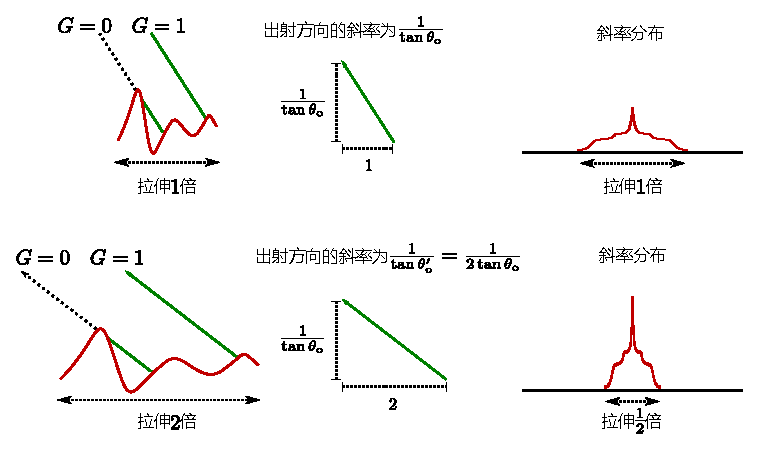
\includegraphics[width=\linewidth]{Pictures/chap08/Stretch1D.eps}
    \caption{一维微面结构的拉伸}
    \label{fig:08ex01-Stretch1D}
\end{figure}

现在,我们显式地把粗糙度参数$\alpha$(或分别在$x$和$y$方向上的$\alpha_x$、$\alpha_y$)
引入微面分布函数和斜率分布(实际上它已提前出现在\reftab{08ex01-Beckmann-V-cavity-Smith-Table}中了)。
回顾上节内容,尤其是\refeq{08-ex01-slope-of-surface}、\refeq{08-ex01-normals-by-slope}、
\refeq{08-ex01-normal-of-P2D}和\refeq{08-ex01-relation-P2D-McrofacetDistribution},我们拓展两者的记号:
对于各向同性分布,分别重新记作$D({\bm\omega}_{\mathrm{h}},\alpha)$和$P_{xy}(x_s,y_s,\alpha)$;
对于各向异性分布,分别重新记作$D({\bm\omega}_{\mathrm{h}},\alpha_x,\alpha_y)$和$P_{xy}(x_s,y_s,\alpha_x,\alpha_y)$.

\subsubsection*{各向同性斜率分布的形状不变性}
典型的各向同性参数化斜率分布依赖粗糙度参数$\alpha$,改变$\alpha$等价于拉伸分布而不改变其形状。
这种情形下,斜率分布只决定于斜率大小$\displaystyle\tan\theta=\sqrt{x_s^2+y_s^2}$(也即
微面法线天顶角正切值)与$\alpha$的比例$\displaystyle\frac{\tan\theta}{\alpha}$:
\begin{align}\label{eq:08-ex01-isotropic-shape-invariant}
    P_{xy}(x_s,y_s,\alpha)=\frac{1}{\alpha^2}f\left(\frac{\sqrt{x_s^2+y_s^2}}{\alpha}\right)=\frac{1}{\alpha^2}f\left(\frac{\tan\theta}{\alpha}\right)\, ,
\end{align}
其中$f$是定义分布形状的一维函数。这样的斜率分布具有\keyindex{形状不变性}{shape invariant}{}:对于任意系数$\lambda>0$,
\begin{align}\label{eq:08-ex01-any-coef-invariant}
    P_{xy}(x_s,y_s,\alpha)=\frac{1}{\lambda^2}P_{xy}(\frac{x_s}{\lambda},\frac{y_s}{\lambda},\frac{\alpha}{\lambda})
\end{align}
恒成立。这意味着它总是具有同样的形状$f$,只由粗糙度参数拉伸和缩放,
且不改变规范性\sidenote{读者可以推导一下。}。

从\reffig{08ex01-Stretch1D}中我们还能看出,因为拉伸操作等价于
把粗糙度参数$\alpha$和出射方向斜率$\displaystyle\frac{1}{\tan\theta_{\mathrm{o}}}$乘以相同系数,
且不会改变光线遮挡关系,所以掩模函数只决定于二者的比值
即$\displaystyle a=\frac{1}{\alpha\tan\theta_{\mathrm{o}}}$.
这也是为什么具有形状不变性的Beckmann-Spizzichino模型和GGX模型各自对应的函数$\Lambda$都只依赖于$a$的原因。
具体而言,对于Beckmann-Spizzichino模型\citep{1987BeckmannSpizzichino},其斜率分布为
\begin{align}
    P_{xy}(x_s,y_s,\alpha)=\frac{1}{\pi\alpha^2}\exp\left(-\frac{x_s^2+y_s^2}{\alpha^2}\right)\, .
\end{align}
将其带入\refeq{08-ex01-relation-P2D-McrofacetDistribution},
并取正向的法线\sidenote{回顾\refeq{08-ex01-normals-by-slope}的批注。},可得
\begin{align}
    D({\bm\omega}_{\mathrm{h}},\alpha)=\frac{\chi({\bm\omega}_{\mathrm{h}}\cdot{\bm\omega}_{\mathrm{g}})}
    {\pi\alpha^2\cos^4\theta}\exp\left(-\frac{\tan^2\theta}{\alpha^2}\right)\, .
\end{align}
最后结合\refeq{08-ex01-condition-1d-slope}和\refeq{08-ex01-Lambda-function},得到
\begin{align}\label{eq:08-ex01-Beckmann-Lambda}
    \Lambda({\bm\omega}_{\mathrm{o}},\alpha)= &\frac{1}{\cot\theta_{\mathrm{o}}}
    \int_{\cot\theta_{\mathrm{o}}}^{+\infty}(x_s-\cot\theta_{\mathrm{o}})P_x(x_s)\mathrm{d}x_s\nonumber \\
    =&\frac{1}{\cot\theta_{\mathrm{o}}}\int_{\cot\theta_{\mathrm{o}}}^{+\infty}
    (x_s-\cot\theta_{\mathrm{o}})\left(\int_{-\infty}^{+\infty}P_{xy}(x_s,y_s)\mathrm{d}y_s\right)\mathrm{d}x_s\nonumber \\
    =&\frac{1}{\cot\theta_{\mathrm{o}}}\int_{\cot\theta_{\mathrm{o}}}^{+\infty}
    (x_s-\cot\theta_{\mathrm{o}})\left(\int_{-\infty}^{+\infty}\frac{1}{\pi\alpha^2}
    \exp\left(-\frac{x_s^2+y_s^2}{\alpha^2}\right)\mathrm{d}y_s\right)\mathrm{d}x_s\nonumber \\
    =&\frac{1}{\pi\cot\theta_{\mathrm{o}}}\int_{\cot\theta_{\mathrm{o}}}^{+\infty}
    (x_s-\cot\theta_{\mathrm{o}})\mathrm{e}^{-\frac{x_s^2}{\alpha^2}}
    \left(\int_{-\infty}^{+\infty}\mathrm{e}^{-\frac{y_s^2}{\alpha^2}}
    \mathrm{d}\frac{y_s}{\alpha}\right)\mathrm{d}\frac{x_s}{\alpha}\nonumber\\
    =&\frac{1}{\pi\cot\theta_{\mathrm{o}}}\int_{\cot\theta_{\mathrm{o}}}^{+\infty}
    \sqrt{\pi}(x_s-\cot\theta_{\mathrm{o}})\mathrm{e}^{-\frac{x_s^2}{\alpha^2}}
    \mathrm{d}\frac{x_s}{\alpha}\nonumber\\
    \xlongequal{\text{令}x=\frac{x_s}{\alpha}}&\frac{1}{\sqrt{\pi}\cot\theta_{\mathrm{o}}}
    \int_{\frac{1}{\alpha\tan\theta_{\mathrm{o}}}}^{+\infty}
    (\alpha x-\cot\theta_{\mathrm{o}})\mathrm{e}^{-x^2}\mathrm{d}x\nonumber\\
    \xlongequal{\text{令}a=\frac{1}{\alpha\tan\theta_{\mathrm{o}}}}&\frac{1}{\sqrt{\pi}a}
    \int_{a}^{+\infty}x\mathrm{e}^{-x^2}\mathrm{d}x
    -\frac{1}{\sqrt{\pi}}\int_{a}^{+\infty}\mathrm{e}^{-x^2}\mathrm{d}x\nonumber\\
    =&\frac{1}{\sqrt{\pi}a}\int_{a}^{+\infty}\frac{-1}{2}\mathrm{d}\mathrm{e}^{-x^2}
    -\frac{1}{\sqrt{\pi}}\left(\int_{0}^{+\infty}\mathrm{e}^{-x^2}\mathrm{d}x
    -\int_{0}^{a}\mathrm{e}^{-x^2}\mathrm{d}x\right)\nonumber\\
    =&\frac{1}{2\sqrt{\pi}a}\mathrm{e}^{-a^2}-\frac{1}{\sqrt{\pi}}
    \left(\frac{\sqrt{\pi}}{2}-\frac{\sqrt{\pi}}{2}\mathrm{erf}(a)\right)\nonumber\\
    =&\frac{1}{2}\left(\mathrm{erf}(a)-1+\frac{\mathrm{e}^{-a^2}}{\sqrt{\pi}a}\right)\, ,
\end{align}
其中使用了误差函数$\displaystyle\mathrm{erf}(a)=\frac{2}{\sqrt{\pi}}\int_{0}^{a}\mathrm{e}^{-x^2}\mathrm{d}x$.
由于该模型计算开销大,\citet{10.5555/2383847.2383874}提出了对其
掩模函数$G_1({\bm\omega}_{\mathrm{h}},{\bm\omega}_{\mathrm{o}})$进行简化近似计算的方法,
代入\refeq{08-ex01-Smith-masking-function}后相当于取
\begin{align}\label{eq:08-ex01-approximation-Beckmann}
    \Lambda({\bm\omega}_{\mathrm{o}},\alpha)\approx\left\{\begin{array}{l}
        \displaystyle\frac{1-1.259a+0.396a^2}{3.535a+2.181a^2},\quad\text{若}a>1.6, \\
        0,\quad\text{其他}.
    \end{array}\right.
\end{align}

类似地,对于Trowbridge-Reitz模型\citep{Trowbridge:75},
也称GGX分布\sidenote{根据\citet{Heitz2018GGX}的说法,
“GGX”表示“ground glass unknown”,未知的磨砂玻璃。}\citep{10.5555/2383847.2383874},
其斜率分布和微面分布函数分别为
\begin{align}
    P_{xy}(x_s,y_s,\alpha)=&\frac{1}{\displaystyle\pi\alpha^2\left(1+\frac{x_s^2+y_s^2}{\alpha^2}\right)^2}\, ,\\
    D({\bm\omega}_{\mathrm{h}},\alpha)=&\frac{\chi({\bm\omega}_{\mathrm{h}}\cdot{\bm\omega}_{\mathrm{g}})}
    {\displaystyle\pi\alpha^2\left(1+\frac{\tan^2\theta}{\alpha^2}\right)^2\cos^4\theta}\, .
\end{align}
仿照\refeq{08-ex01-Beckmann-Lambda}的推导,可得
\begin{align}\displaystyle
    \Lambda({\bm\omega}_{\mathrm{o}},\alpha)=&\frac{1}{\cot\theta_{\mathrm{o}}}\int_{\cot\theta_{\mathrm{o}}}^{+\infty}
    (x_s-\cot\theta_{\mathrm{o}})\left(\int_{-\infty}^{+\infty}
    \frac{1}{\displaystyle\pi\alpha^2\left(1+\frac{x_s^2+y_s^2}{\alpha^2}\right)^2}\mathrm{d}y_s\right)\mathrm{d}x_s\nonumber \\
    =&\frac{\alpha^2}{\pi\cot\theta_{\mathrm{o}}}\int_{\cot\theta_{\mathrm{o}}}^{+\infty}
    (x_s-\cot\theta_{\mathrm{o}})\left(\int_{-\infty}^{+\infty}
    \frac{1}{\displaystyle\left(\alpha^2+x_s^2+y_s^2\right)^2}\mathrm{d}y_s\right)\mathrm{d}x_s\nonumber\\
    =&\frac{\alpha^2}{\pi\cot\theta_{\mathrm{o}}}\int_{\cot\theta_{\mathrm{o}}}^{+\infty}
    (x_s-\cot\theta_{\mathrm{o}})\left(\int_{-\infty}^{+\infty}\frac{1}{\displaystyle
    \left((\alpha^2+x_s^2)\left(1+\frac{y_s^2}{\alpha^2+x_s^2}\right)\right)^2}\mathrm{d}y_s\right)\mathrm{d}x_s\nonumber\\
    =&\frac{\alpha^2}{\pi\cot\theta_{\mathrm{o}}}\int_{\cot\theta_{\mathrm{o}}}^{+\infty}
    \frac{x_s-\cot\theta_{\mathrm{o}}}{(\alpha^2+x_s^2)^\frac{3}{2}}\left(\int_{-\infty}^{+\infty}
    \frac{\displaystyle\mathrm{d}\frac{y_s}{\sqrt{\alpha^2+x_s^2}}}
    {\displaystyle\left(1+\left(\frac{y_s}{\sqrt{\alpha^2+x_s^2}}\right)^2\right)^2}\right)\mathrm{d}x_s\nonumber\\
    \xlongequal{\text{令}t=\frac{y_s}{\sqrt{\alpha^2+x_s^2}}}&\frac{\alpha^2}{\pi\cot\theta_{\mathrm{o}}}
    \int_{\cot\theta_{\mathrm{o}}}^{+\infty}\frac{x_s-\cot\theta_{\mathrm{o}}}{(\alpha^2+x_s^2)^\frac{3}{2}}
    \left(\int_{-\infty}^{+\infty}\frac{\mathrm{d}t}{(1+t^2)^2}\right)\mathrm{d}x_s\nonumber\\
    =&\frac{\alpha^2}{\pi\cot\theta_{\mathrm{o}}}\int_{\cot\theta_{\mathrm{o}}}^{+\infty}
    \frac{x_s-\cot\theta_{\mathrm{o}}}{(\alpha^2+x_s^2)^\frac{3}{2}}\cdot\frac{\pi}{2}\mathrm{d}x_s\nonumber\\
    =&\frac{\alpha^2}{2\cot\theta_{\mathrm{o}}}\int_{\cot\theta_{\mathrm{o}}}^{+\infty}
    \frac{x_s\mathrm{d}x_s}{(\alpha^2+x_s^2)^\frac{3}{2}}-\frac{1}{2}\int_{\cot\theta_{\mathrm{o}}}^{+\infty}
    \frac{\alpha^2\mathrm{d}x_s}{(\alpha^2+x_s^2)^\frac{3}{2}}\nonumber\\
    =&-\frac{\alpha^2}{2\cot\theta_{\mathrm{o}}}\int_{\cot\theta_{\mathrm{o}}}^{+\infty}\mathrm{d}(\alpha^2+x_s^2)^{-\frac{1}{2}}
    -\frac{1}{2}\int_{\cot\theta_{\mathrm{o}}}^{+\infty}\mathrm{d}\frac{x_s}{\sqrt{\alpha^2+x_s^2}}\nonumber\\
    =&-\frac{\alpha^2}{2\cot\theta_{\mathrm{o}}\sqrt{\alpha^2+x_s^2}}\bigg|_{x_s=\cot\theta_{\mathrm{o}}}^{+\infty}
    -\frac{1}{2}\frac{x_s}{\sqrt{\alpha^2+x_s^2}}\bigg|_{x_s=\cot\theta_{\mathrm{o}}}^{+\infty}\nonumber\\
    =&\frac{\alpha^2}{2\cot\theta_{\mathrm{o}}\sqrt{\alpha^2+\cot^2\theta_{\mathrm{o}}}}
    -\frac{1}{2}\left(1-\frac{\cot\theta_{\mathrm{o}}}{\sqrt{\alpha^2+\cot^2\theta_{\mathrm{o}}}}\right)\nonumber\\
    =&\frac{\alpha^2-\cot\theta_{\mathrm{o}}\sqrt{\alpha^2+\cot^2\theta_{\mathrm{o}}}+
    \cot^2\theta_{\mathrm{o}}}{2\cot\theta_{\mathrm{o}}\sqrt{\alpha^2+\cot^2\theta_{\mathrm{o}}}}\nonumber\\
    \xlongequal{\text{令}a=\frac{1}{\alpha\tan\theta_{\mathrm{o}}}}&\frac{\alpha^2-
    a\alpha\sqrt{\alpha^2+a^2\alpha^2}+a^2\alpha^2}{2a\alpha\sqrt{\alpha^2+a^2\alpha^2}}\nonumber\\
    =&\frac{1}{2}(\sqrt{1+a^{-2}}-1)\, .
\end{align}

可以看到,以上两种模型的斜率分布都可以表示为\refeq{08-ex01-isotropic-shape-invariant}的形式,
所以它们具有形状不变性。但要注意的是,不是所有分布都具有形状不变性。

\subsubsection*{各向异性斜率分布的形状不变性}
如果我们按照类似于上小节的方法,改成用与方位相关的参数去拉伸形状,就会得到各向异性版的形状不变性分布。
具体来说,\refeq{08-ex01-isotropic-shape-invariant}将替换为
\begin{align}
    P_{xy}(x_s,y_s,\alpha_x,\alpha_y)=\frac{1}{\alpha_x\alpha_y}f\displaystyle
    \left(\sqrt{\frac{x_s^2}{\alpha_x^2}+\frac{y_s^2}{\alpha_y^2}}\right)
    =\frac{1}{\alpha_x\alpha_y}f\left(\tan\theta\sqrt{\frac{\cos^2\varphi}{\alpha_x^2}
    +\frac{\sin^2\varphi}{\alpha_y^2}}\right)\, ,
\end{align}
其中$\alpha_x$和$\alpha_y$是分布分别在$x$和$y$轴方向上的拉伸系数。
而各向同性版本是它在$\alpha_x=\alpha_y$时的特例。
\refeq{08-ex01-any-coef-invariant}也相应拓展为
\begin{align}
    P_{xy}(x_s,y_s,\alpha_x,\alpha_y)=\frac{1}{\lambda_x\lambda_y}P_{xy}(\frac{x_s}{\lambda_x},\frac{y_s}{\lambda_y},\frac{\alpha_x}{\lambda_x},\frac{\alpha_y}{\lambda_y})
\end{align}
对任意$\alpha_x,\alpha_y>0$恒成立,其规范性也仍然成立。

\reffig{08ex01-2D-Anisotropic-Stretch}展示了一个具有形状不变性的分布是如何通过拉伸
在各向同性和各向异性之间互相转化的。下面我们借助该特性推导各向异性分布的掩模函数。
\begin{figure}[htbp]
    \centering
    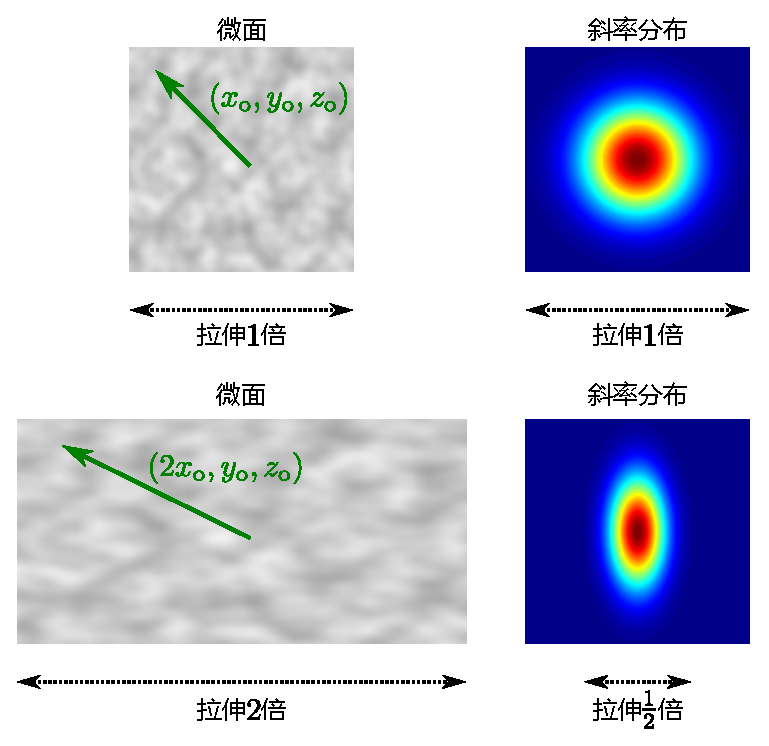
\includegraphics[width=0.8\linewidth]{Pictures/chap08/Anisotropic-Shape-Invariant-Distributions-of-Slopes.eps}
    \caption{二维微面结构通过拉伸在各向同性和各向异性间转化。}
    \label{fig:08ex01-2D-Anisotropic-Stretch}
\end{figure}

对于具有参数$\alpha_x$和$\alpha_y$的各向异性形状不变分布和某
出射方向${\bm\omega}_{\mathrm{o}}=(x_{\mathrm{o}},y_{\mathrm{o}},z_{\mathrm{o}})$,
我们在$x$轴方向上对其拉伸$\displaystyle\frac{\alpha_x}{\alpha_y}$倍,使其变回各向同性版本,
得到新的粗糙度参数、出射向量和斜率分别为
\begin{align}
    \alpha'_x=&\alpha_x\frac{\alpha_y}{\alpha_x}=\alpha_y\, ,\\
    \alpha'_y=&\alpha_y\, ,\\
    {\bm\omega}'_{\mathrm{o}}=&(\frac{\alpha_x}{\alpha_y}x_{\mathrm{o}},y_{\mathrm{o}},z_{\mathrm{o}})
    =(\frac{\alpha_x}{\alpha_y}\cos\varphi_{\mathrm{o}}\sin\theta_{\mathrm{o}},
    \sin\varphi_{\mathrm{o}}\sin\theta_{\mathrm{o}},\cos\theta_{\mathrm{o}})\, ,\\
    \frac{1}{\tan\theta'_{\mathrm{o}}}=&\frac{z_{\mathrm{o}}}
    {\sqrt{\displaystyle\frac{\alpha_x^2}{\alpha_y^2}x_{\mathrm{o}}^2+y_{\mathrm{o}}^2}}
    =\frac{1}{\tan\theta_{\mathrm{o}}\sqrt{\displaystyle\frac{\alpha_x^2}{\alpha_y^2}\cos^2\varphi_{\mathrm{o}}+\sin^2\varphi_{\mathrm{o}}}}\, .
\end{align}
对于拉伸后的各向同性分布,对应的新比率参数为
\begin{align}
    a'=&\frac{1}{\alpha'_y\tan\theta'_{\mathrm{o}}}\nonumber\\
      =&\frac{1}{\alpha_y\tan\theta_{\mathrm{o}}\sqrt{\displaystyle\frac{\alpha_x^2}{\alpha_y^2}\cos^2\varphi_{\mathrm{o}}+\sin^2\varphi_{\mathrm{o}}}}\nonumber\\
      =&\frac{1}{\tan\theta_{\mathrm{o}}\sqrt{\alpha_x^2\cos^2\varphi_{\mathrm{o}}+\alpha_y^2\sin^2\varphi_{\mathrm{o}}}}\nonumber\\
      =&\frac{1}{\alpha_{\mathrm{o}}\tan\theta_{\mathrm{o}}}\, ,
\end{align}
其中
\begin{align}
    \alpha_{\mathrm{o}}=\sqrt{\alpha_x^2\cos^2\varphi_{\mathrm{o}}+\alpha_y^2\sin^2\varphi_{\mathrm{o}}}
\end{align}
定义为投影到出射方向的粗糙度。这说明各向异性的形状不变斜率分布的掩模函数和各向同性的有相同本质,
唯一的区别在于前者由各向异性曲面投影到出射方向上的粗糙度来进行参数化
\sidenote{理解这句话才能理解为什么各向异性版的$\Lambda$形式几乎不变。}。
利用该性质,我们可以给出以下两个各向异性模型的掩模函数:

对于Beckmann-Spizzichino模型,其各向异性分布为
\begin{align}
    P_{xy}(x_s,y_s,\alpha_x,\alpha_y)=&\frac{1}{\pi\alpha_x\alpha_y}\exp\left(-\frac{x_s^2}{\alpha_x^2}-\frac{y_s^2}{\alpha_y^2}\right)\, ,\\
    D({\bm\omega}_{\mathrm{h}},\alpha_x,\alpha_y)=&\frac{\chi({\bm\omega}_{\mathrm{h}}\cdot{\bm\omega}_{\mathrm{g}})}
    {\pi\alpha_x\alpha_y\cos^4\theta}\exp\left(-\left(\frac{\cos^2\varphi}{\alpha_x^2}
    +\frac{\sin^2\varphi}{\alpha_y^2}\right)\tan^2\theta\right)\, ,\\
    \Lambda({\bm\omega}_{\mathrm{o}},\alpha_x,\alpha_y)=&\frac{1}{2}\left(\mathrm{erf}(a)-1
    +\frac{\mathrm{e}^{-a^2}}{\sqrt{\pi}a}\right),
    \quad\text{其中}a=\displaystyle\frac{1}{\alpha_{\mathrm{o}}\tan\theta_{\mathrm{o}}}\, .
\end{align}
且\refeq{08-ex01-approximation-Beckmann}的近似计算方法仍然适用。

对于Trowbridge-Reitz模型,其各向异性分布为
\begin{align}
    P_{xy}(x_s,y_s,\alpha_x,\alpha_y)=&\frac{1}{\displaystyle\pi\alpha_x\alpha_y\left(1
    +\frac{x_s^2}{\alpha_x^2}+\frac{y_s^2}{\alpha_y^2}\right)^2}\, ,\\
    D({\bm\omega}_{\mathrm{h}},\alpha_x,\alpha_y)=&\frac{\chi({\bm\omega}_{\mathrm{h}}\cdot{\bm\omega}_{\mathrm{g}})}
    {\displaystyle\pi\alpha_x\alpha_y\left(1+\left(\frac{\cos^2\varphi}{\alpha_x^2}
    +\frac{\sin^2\varphi}{\alpha_y^2}\right)\tan^2\theta\right)^2\cos^4\theta}\, ,\\
    \Lambda({\bm\omega}_{\mathrm{o}},\alpha_x,\alpha_y)=&\frac{1}{2}(\sqrt{1+a^{-2}}-1),
    \quad\text{其中}a=\displaystyle\frac{1}{\alpha_{\mathrm{o}}\tan\theta_{\mathrm{o}}}\, .
\end{align}

我们还可以分别验证下以上两个模型是否满足规范性即\refeq{08-ex01-normal-of-P2D},对于Beckmann-Spizzichino模型有:
\begin{align}
    &\int_{-\infty}^{+\infty}\int_{-\infty}^{+\infty}\frac{1}{\pi\alpha_x\alpha_y}\exp\left(-\frac{x_s^2}{\alpha_x^2}-\frac{y_s^2}{\alpha_y^2}\right)\mathrm{d}x_s\mathrm{d}y_s\nonumber\\
    =&\frac{1}{\pi}\left(\int_{-\infty}^{+\infty}\mathrm{e}^{-\frac{x_s^2}{\alpha_x^2}}\frac{\mathrm{d}x_s}{\alpha_x}\right)\left(\int_{-\infty}^{+\infty}\mathrm{e}^{-\frac{y_s^2}{\alpha_y^2}}\frac{\mathrm{d}y_s}{\alpha_y}\right)\nonumber\\
    =&\frac{1}{\pi}\cdot\sqrt{\pi}\cdot\sqrt{\pi}=1\, .
\end{align}
对于Trowbridge-Reitz模型,注意到积分式
\begin{align}
    \int\frac{\mathrm{d}x}{(b^2+x^2)^2}=\frac{x}{2b^2(b^2+x^2)}+\frac{1}{2b^3}\arctan\frac{x}{b}+C\, ,
\end{align}
于是有
\begin{align}
    &\int_{-\infty}^{+\infty}\int_{-\infty}^{+\infty}\frac{1}{\displaystyle\pi\alpha_x\alpha_y\left(1
    +\frac{x_s^2}{\alpha_x^2}+\frac{y_s^2}{\alpha_y^2}\right)^2}\mathrm{d}x_s\mathrm{d}y_s\nonumber\\
    \xlongequal{\text{令}x=\frac{x_s}{\alpha_x},y=\frac{y_s}{\alpha_y}}&\int_{-\infty}^{+\infty}\int_{-\infty}^{+\infty}
    \frac{1}{\pi\left(1+x^2+y^2\right)^2}\mathrm{d}x\mathrm{d}y\nonumber\\
    =&\frac{1}{\pi}\int_{-\infty}^{+\infty}\left(\frac{x}{2(1+y^2)(1+x^2+y^2)}
    +\frac{1}{2(1+y^2)^{\frac{3}{2}}}\arctan\frac{x}{\sqrt{1+y^2}}\right)
    \bigg|_{x=-\infty}^{+\infty}\mathrm{d}y\nonumber\\
    =&\frac{1}{\pi}\int_{-\infty}^{+\infty}\frac{\pi}{2(1+y^2)^{\frac{3}{2}}}\mathrm{d}y\nonumber\\
    =&\frac{1}{2}\int_{-\infty}^{+\infty}\mathrm{d}\frac{y}{\sqrt{1+y^2}}\nonumber\\
    =&\frac{1}{2}\frac{y}{\sqrt{1+y^2}}\bigg|_{y=-\infty}^{+\infty}=1\, .
\end{align}
由此它们的$D({\bm\omega}_{\mathrm{h}},\alpha_x,\alpha_y)$也满足规范性。